% LREC 2026 Example; 
% LREC Is now using templates similar to the ACL ones. 
\documentclass[10pt, a4paper]{article}
\usepackage{multirow}
\usepackage{lrec2026} 
\usepackage{microtype}
\usepackage{hyperref}
\usepackage{xurl}
\usepackage{booktabs}
\usepackage{subfigure}
\usepackage[switch]{lineno}
\makeatletter
\providecommand{\@LN@col}[1]{}
\makeatother
\usepackage{natbib}
\usepackage{multibib}
% \newcites{lr}{Language Resources References}
\newcites{lr}{\ }
% \usepackage{CJK}
\usepackage{CJKutf8}
\usepackage{array}
\usepackage{makecell}
\usepackage{rotating}
\usepackage{ulem} 
\usepackage{comment}
\usepackage{graphicx}
\definecolor{darkblue}{rgb}{0, 0, 0.5}
\hypersetup{colorlinks=true, citecolor=darkblue, linkcolor=darkblue, urlcolor=darkblue}
\usepackage{fvextra} 
\RecustomVerbatimEnvironment{verbatim}{Verbatim}{
  breaklines=true,
  breakanywhere=true,   
  fontsize=\small,      
  obeytabs=true       
}
\usepackage{titlesec}
\titleclass{\subsubsubsection}{straight}[\subsubsection]
\newcounter{subsubsubsection}[subsubsection]
\renewcommand\thesubsubsubsection{\thesubsubsection.\arabic{subsubsubsection}}
\titleformat{\subsubsubsection}
  {\normalfont\normalsize\bfseries}{\thesubsubsubsection}{1em}{}
\titlespacing*{\subsubsubsection}
  {0pt}{1ex plus 0.5ex}{0.5ex}
% this is the new style
% the 'review' option anonymizes the paper following submission guideline
% the 'final' option produces the camera ready version (non anonymized)
% default version is 'final', so use review option for submission
\usepackage{float}

\hyphenation{macOS}

%\title{Benchmarking Large Language Models for Text Input in Chinese and Japanese} 
\title{Benchmarking Large Language Models for Chinese and Japanese IMEs: Phonetic-to-Character Generation and Textual Error Correction}
%TODO: use this title if change is allowed

\name{Yuchun Zou$^{\ast}$, Tedd Lee$^{\S}$, Xiaodi Fan$^{\ddagger}$, Jun Li$^{\dagger}$}

\address{$^{\ast}$CUNY Graduate Center, New York, NY \\
         \texttt{yzou@gradcenter.cuny.edu} \\
         $^{\S}$CUNY Hunter College, New York, NY \\
         \texttt{tedd.lee69@myhunter.cuny.edu} \\
         $^{\ddagger}$Meta Inc., New York, NY \\
         \texttt{xfan@meta.com} \\
         $^{\dagger}$CUNY Queens College \& Graduate Center, New York, NY \\
         \texttt{junli@qc.cuny.edu} \\
         }

\abstract{
Efficient text entry for complex writing systems like Chinese and Japanese necessitates the use of Input Method Editors (IMEs). While Large Language Models (LLMs) are emerging as powerful, context-aware language resources for this task, we present a comprehensive benchmark and evaluation methodology to assess the viability of LLMs for next-generation IMEs. We conduct a comparative analysis of a diverse set of LLMs against established baseline methods on two core tasks: phonetic-to-character generation (using Pinyin and Romaji) and textual error correction. Our experiments demonstrate that top-tier LLMs achieve superior accuracy by leveraging deep contextual understanding, significantly outperforming traditional systems in ambiguity resolution and the correction of complex errors. However, our analysis also reveals a crucial trade-off between accuracy and computational efficiency across different models. The datasets, evaluation scripts, and results from this study serve as a vital public resource for future research, providing a robust baseline for developing and selecting models that balance performance with the low-latency demands of real-world text input.
 \\ \newline \Keywords{Benchmarking, Input Method Editor (IME), Large Language Model, Chinese, Japanese}}

\begin{document}
\maketitleabstract


\section{Introduction}
Text input for languages with complex writing systems like Chinese and Japanese presents a unique and persistent challenge. Unlike alphabetic languages, which primarily rely on a one-to-one mapping between keystrokes and characters, these systems employ thousands of logographic characters, making direct keyboard entry impractical. This necessitates the use of Input Method Editors (IMEs), specialized software that serves as the crucial bridge between a standard keyboard and the target script. The core function of an IME is to convert phonetic input, such as Pinyin for Mandarin Chinese or Romaji for Japanese, into the intended characters. This process is far from straightforward, primarily due to the pervasive homophony in these languages, where a single pronunciation can correspond to many different characters.

% Current IMEs predominantly rely on statistical models, such as n-grams \citep{Li2015}, and rule-based systems \citep{Goh2005} to disambiguate phonetic input. While functional, these methods suffer from significant limitations rooted in their narrow contextual understanding. Operating on a local word-by-word or character-by-character basis, they often fail to capture the subtle semantic cues required for accurate disambiguation in longer sentences or less common phrases. 

% Current Input Method Editors (IMEs) have evolved significantly beyond early rule-based systems \citep{goh2005}. The foundational statistical models, which relied on local word segmentation and n-gram frequencies, provided the initial framework for these tools \citep{gao2002improving}. More advanced approaches later incorporated neural network architectures like Recurrent Neural Networks (RNNs) to better model sequential dependencies \citep{li2015}. 
% Furthermore, state-of-the-art research has demonstrated that enhancing these neural IMEs with powerful contextualized embeddings from pre-trained encoder models like BERT can further improve disambiguation accuracy \citep{meng2021contextual}. 
% This paradigm of using pre-trained models culminated in the development of powerful, language-specific architectures like ChineseBERT, which leverages deep contextual understanding to achieve state-of-the-art results on related disambiguation tasks such as Chinese spelling correction \citep{sun2021chinesebert}.

The evolution of Input Method Editors (IMEs) provides a clear technological progression. Early systems were often rule-based \citep{goh2005}, but the dominant paradigm for years has been based on statistical models. Tools like {Pinyin2Hanzi} \citep{pinyin2hanzi}, which uses n-gram frequencies, are prime examples of this foundational approach \citep{gao2002improving}. A significant step forward came with the incorporation of neural network architectures like Recurrent Neural Networks (RNNs) to better model sequential dependencies \citep{chen2015neural}. This neural paradigm culminated in powerful, specialized models like ChineseBERT, which leverage deep contextual understanding to achieve state-of-the-art results on related tasks like Chinese Spelling Correction \citep{sun2021chinesebert}, a principle shared by modern correction tools like {pycorrector} \citep{pycorrector}. 

Despite these advances, a fundamental paradigm remains: these systems function primarily as sophisticated ranking models. Their core task is to disambiguate phonetic input by selecting the most probable character or word from a pre-defined candidate list, based on the immediate local context~\citep{sun2021chinesebert,chen2015neural}. Even when enhanced with contextual embeddings, their reasoning is still fundamentally rooted in this local disambiguation task. They often fail to capture the long-range semantic and pragmatic cues required for high-fidelity composition in complex sentences.
Furthermore, their error-correction capabilities are rudimentary. They are typically designed to handle simple typographical errors but are ill-equipped to address more complex issues that users frequently encounter, such as homophone confusion, phonetic misspellings, or semantic incongruities~\citep{tseng2015introduction}. These shortcomings hinder input speed and degrade the overall user experience, necessitating frequent manual corrections.

Large Language Models (LLMs), with their demonstrated proficiency across a wide range of NLP tasks \citep{bommasani2021opportunities, zhao2023survey, zhou2023comprehensive}, offer a promising new paradigm for IME technology. Trained on vast text corpora, LLMs function as powerful language resources capable of learning and leveraging intricate and long-range context. This deep understanding allows them to address the core weaknesses of traditional IMEs. By considering the entire sentence or discourse, LLMs can disambiguate homophones with far greater accuracy and generate more natural-sounding text. Moreover, their capacity for learning complex linguistic patterns enables them to identify and correct a much wider spectrum of user errors, moving beyond simple typos to address mistakes in phonetics and semantics.

This paper introduces a comprehensive benchmark to systematically evaluate the performance of LLMs as a foundational technology for next-generation Chinese and Japanese IMEs. Our primary contribution is a rigorous comparative analysis of a diverse range of LLMs against established baselines on two fundamental tasks: (1) phonetic-to-character generation and (2) textual error correction. To ensure a thorough and robust evaluation, we assess model performance using a comprehensive suite of metrics. This includes measures for semantic similarity (SimHash, BERTScore~\citep{zhang2019bertscore}), lexical accuracy (BLEU~\citep{papineni2002bleu}, ROUGE~\citep{lin2004rouge}), and character error rate (CER), all weighed against computational efficiency (completion time, time to first token (TTFT), and tokens per second (TPS)). While performance varies across different LLMs, the overall trend indicates significant potential for enhanced accuracy and a more natural user experience compared to existing IMEs. Moreover, this multi-faceted evaluation provides crucial, nuanced insights into the trade-offs between linguistic fidelity and processing speed, establishing a robust methodology and public resource for developing and benchmarking future IME technologies.


\section{Related Works}

The application of Large Language Models (LLMs) to specialized language technology tasks has become a central theme in recent research \citep{bommasani2021opportunities, zhao2023survey}. While foundational models like BERT \citep{devlin2018bert} and GPT-2 \citep{radford2019language} set the stage for advanced text generation, their application to the nuanced challenges of Input Method Editors (IMEs) for complex scripts like Chinese and Japanese remains a nascent field of study. This section reviews prior work in phonetic-to-character generation and textual error correction, highlighting the gaps that motivate our comprehensive benchmark.

\textbf{LLMs in Phonetic-to-Character Generation.}
Pioneering studies have explored the integration of LLMs with phonetic input systems. For example, \citet{sun2021chinesebert} integrated a GPT model with a Pinyin IME, and \citet{tan2022exploring} investigated large-scale pre-training for Pinyin-based text generation. These efforts have been limited in scope, primarily focusing on Chinese without a comparative analysis across a wide range of LLMs or extension to other complex scripts like Japanese. Furthermore, their main objective was text generation, with limited attention to the critical, real-world task of correcting user errors. Finally, the practical usability of any IME is governed by latency, a factor explored in general text generation \citep{stahlberg2020neural, brown2020language} but one that requires specific evaluation in the context of interactive text input.

\textbf{Textual Error Correction.}
% In the parallel domain of textual error correction, significant progress has been made using neural architectures for languages like Persian and Arabic \citep{dashti2024percore, alkhatib2020deep, kasmaiee2023correcting}. However, these approaches are not directly transferable to Chinese and Japanese. The linguistic challenges are fundamentally different: the high degree of homophony and the complex, multi-script character systems of Chinese and Japanese necessitate error correction strategies that are deeply sensitive to both phonetic and semantic context. A simple character-level correction model for a largely phonetic script cannot resolve the ambiguity of a user selecting the wrong homophonous character (\textit{e.g.}, \begin{CJK}{UTF8}{gbsn}的\end{CJK} vs. \begin{CJK}{UTF8}{gbsn}地\end{CJK} in Chinese), a common error that requires contextual understanding.
In the parallel domain of textual error correction, significant progress has been made using neural architectures for languages like Persian and Arabic \citep{dashti2024percore, alkhatib2020deep, kasmaiee2023correcting}. However, these approaches are not directly transferable to Chinese and Japanese. The linguistic challenges are fundamentally different: the high degree of homophony and the complex, multi-script character systems of Chinese and Japanese necessitate error correction strategies that are deeply sensitive to both phonetic and semantic context. A simple character-level correction model for a largely phonetic script cannot resolve the ambiguity of a user selecting the wrong homophonous character. For example, choosing between the possessive particle \begin{CJK*}{UTF8}{gbsn}的\end{CJK*} (\textit{d\'{e}}) and the adverbial particle \begin{CJK*}{UTF8}{gbsn}地\end{CJK*} (\textit{d\'{e}}) in Chinese, a common error that requires syntactic and semantic understanding of the entire sentence.

\textbf{The Need for a Comprehensive Benchmark.}
This review reveals a clear gap in the literature: the absence of a comprehensive, multi-faceted benchmark for evaluating LLMs as a resource for Chinese and Japanese IMEs. Existing work tends to focus on a single language \citep{sun2021chinesebert, sawada2024release}, a single task (generation or correction), or a limited set of models \citep{suvarna2023phonologybench}. This narrow focus extends even to powerful multilingual models like XLM-R \citep{conneau-etal-2020-unsupervised}, whose evaluations have centered on broad cross-lingual understanding benchmarks (e.g., XNLI) rather than the fine-grained, interactive task of phonetic-to-character selection required for IMEs. Our research directly addresses these gaps by establishing the first benchmark that systematically evaluates a diverse range of LLMs, including multilingual, open-source, and proprietary models, across both phonetic-to-character generation and textual error correction for both Chinese and Japanese. By employing a robust suite of evaluation metrics, we provide a much-needed, holistic view of the potential and limitations of LLMs for this critical application.

\section{Linguistic and Input Challenges}

% The design of effective IMEs for Chinese and Japanese is dictated by the unique linguistic properties of their writing systems. We frame these properties as two primary computational challenges that any advanced IME must overcome: inherent linguistic ambiguity and the prevalence of user input errors.

\subsection{The Challenge of Inherent Ambiguity}
Both Chinese and Japanese are characterized by a high degree of homophony, making phonetic input inherently ambiguous.

{In Chinese,} the logographic writing system (Hanzi) requires a phonetic input method like Pinyin. The core challenge arises from the many-to-one mapping of characters to pronunciations. For example, the Pinyin input ``yì yì'' could correspond to entirely different meaningful phrases such as \begin{CJK*}{UTF8}{gbsn}意义\end{CJK*} (meaning/significance) or \begin{CJK*}{UTF8}{gbsn}异议\end{CJK*} (objection). Similarly, ``tā men'' could refer to \begin{CJK*}{UTF8}{gbsn}他们\end{CJK*} (they, male/mixed), \begin{CJK*}{UTF8}{gbsn}她们\end{CJK*} (they, female), or \begin{CJK*}{UTF8}{gbsn}它们\end{CJK*} (they, non-human). This ambiguity requires an IME to perform complex contextual disambiguation, as the correct character sequence can only be predicted by understanding the surrounding text.

{The Japanese writing system} presents an even greater level of complexity by integrating three distinct scripts: Kanji (logographic characters, \textit{e.g.}, \begin{CJK*}{UTF8}{min}木\end{CJK*} for ``tree''), Hiragana (a phonetic syllabary, \textit{e.g.}, \begin{CJK*}{UTF8}{min}き\end{CJK*} for ``ki''), and Katakana (a second syllabary, primarily for loanwords). A user typing the Romaji ``ki'' would first see it converted to Hiragana (\begin{CJK*}{UTF8}{min}き\end{CJK*}). From there, they must select the correct Kanji from a list of homophonous candidates, which could include \begin{CJK*}{UTF8}{min}木\end{CJK*} (tree), \begin{CJK*}{UTF8}{min}気\end{CJK*} (spirit), or \begin{CJK*}{UTF8}{min}機\end{CJK*} (machine). Consequently, contextual disambiguation is a fundamental and pervasive challenge in Japanese text input as well.

\subsection{The Challenge of User Input Errors}
Beyond inherent linguistic ambiguity, a robust IME must also handle a wide range of input errors. These errors can be broadly categorized, starting with {typographical errors}, i.e., simple mistakes in keystrokes such as typing \textit{``xianzia''} instead of \textit{``xianzai''} in Pinyin. Next are {phonetic errors}, which involve using an incorrect Pinyin or Romaji spelling due to a misunderstanding of the pronunciation. Finally, and most challenging for traditional systems, are {orthographic/semantic errors}. These occur when a user selects the wrong character from the IME's candidate list of homophones, even if the phonetic input was correct, resulting in a phonetically valid but semantically incorrect sentence.

Traditional IMEs attempt to address these challenges using mechanisms based on edit distance or simple phonetic similarity rules \citep{wagner1974string, jurafsky2000speech, gao2002improving}. While effective for minor typos, they falter when faced with complex errors, particularly orthographic/semantic mistakes, as they fundamentally lack deep semantic understanding. A traditional IME is unlikely to detect that a user has chosen a contextually inappropriate character if that character is a valid homophone. This dual challenge of resolving deep linguistic ambiguity and correcting multi-layered user errors necessitates models with sophisticated contextual reasoning capabilities, which is precisely the strength of Large Language Models.

\section{Methodology}
\label{sec:methodology}

In this section, we present the methodology for our benchmark of LLMs as advanced IMEs for Chinese and Japanese. We focus on two primary tasks: phonetic-to-character generation and textual error correction. 
% For each task, we detail the data preparation, experimental setup, and evaluation procedures.

\subsection{Task 1: Phonetic-to-Character Generation}

This task assesses the ability of LLMs and baseline methods to accurately convert phonetic input (Pinyin for Chinese, Romaji for Japanese) into the corresponding written characters (Hanzi for Chinese, Kanji/Hiragana/Katakana for Japanese).

\textbf{Datasets.}
For Chinese, we utilized two datasets: one for words from the Phrase Pinyin Data repository \citeplr{phrase-pinyin-data} and one for sentences from the widely-used \textbf{SIGHAN 2015 bake-off} corpus \citep{tseng2015introduction}. For Japanese, we used datasets of words from the Yomichan JLPT vocabulary collection \citeplr{stephenmk2024yomichan} and sentences from the Snow Simplified Japanese Corpus \citeplr{snow2024simplified}. All sentences were preprocessed by converting them to their respective romanizations (Pinyin/Romaji) and removing punctuation.

\textbf{Models and Baselines.}
Our model selection was guided by the specific requirements of real-time IME applications, prioritizing a balance of high performance and low latency. We intentionally chose models optimized for fast text generation and completion. Consequently, we excluded models primarily designed for complex, multi-step reasoning (e.g., Gemini 2.5 Pro and GPT-5 family models), as their typically longer inference times and higher computational overhead are less suitable for the interactive, low-latency demands of text input.

% Our benchmark was designed to be comprehensive within these constraints, covering a wide array of models as detailed in Table~\ref{tab:models_all_scope}. This includes leading proprietary online models, popular open-source offline models, and language-specific models.
Our benchmark covers a wide array of models as detailed in Table~\ref{tab:models_all_scope}, including proprietary models accessed via an API (\textit{online}) and open-weight models deployed locally (\textit{offline}).\footnote{We use the terms {online} and {offline} to classify the \textit{deployment method} for our evaluation, as this distinction is critical for analyzing performance in an interactive application. {Online} models (accessed via API) are subject to network latency, and {offline} models (run locally) are only limited by local compute speed. This is a more direct measure of real-world usability for an IME than the standard proprietary vs. open-weight classification, which describes a model's license rather than its deployment.}

\begin{table}[h!]
\centering
\small
\begin{tabular}{p{1.5cm} p{5.3cm}}
\hline
\textbf{Category} & \textbf{Models Evaluated in Full Study} \\
\hline
Online LLMs & GPT-4, GPT-4o, GPT-4o-mini, Gemini 2.0/2.5 Flash, Claude 3 Sonnet, Claude 3.5 Haiku \\
\hline
Offline LLMs & Llama3-8B, Llama3.2-3B, Mistral-7B, GLM4-9B \\
\hline
Language-Specific LLMs & Qwen2-7B, Baichuan2-7B (Chinese); Rinna Nekomata-7B, RakutenAI-7B, RakutenAI 2.0-mini-1.5B, Swallow-8B (Japanese) \\
\hline
Baseline Methods & macOS Pinyin, macOS Romaji, {Pinyin2Hanzi} (HMM \& DAG), {pycorrector}, {OpenNMT} \\
\hline
\end{tabular}
\caption{The comprehensive set of models and baselines evaluated in our study, selected for their suitability for low-latency text generation tasks.}
\label{tab:models_all_scope}
\end{table}

Exact model versions and API identifiers are listed in Appendix Table~\ref{tab:appendix_models_all}.

While all models in Table~\ref{tab:models_all_scope} were evaluated, for clarity and brevity in our main analysis (Section~\ref{sec:results}), we focus on an analysis subset. This subset includes: GPT-4o-mini (for word generation), GPT-4 (for sentence generation), Gemini 2.0 Flash, Llama3.2-3B, the macOS IMEs, and Pinyin2Hanzi. We selected this subset to cover strong proprietary models, an efficient local model, and established IME baselines, so that core accuracy-latency trade-offs are easy to interpret in the main text.
A comprehensive breakdown of results across all evaluated models and metrics will be provided in the Appendix in the final version of the paper.

\textbf{Implementation Details.}
LLMs were instructed using carefully designed zero-shot prompts with the {temperature} parameter set to 0.1 for more deterministic outputs. Offline models were deployed on a Google Colab instance with an NVIDIA A100 GPU. Baselines included the {Pinyin2Hanzi} library \citep{pinyin2hanzi} including both {HMM} (Hidden Markov Model) and {DAG} (Directed Acyclic Graph) methods, and native system IMEs on macOS, for which we simulated user input via the {keyboard} library \citep{keyboard} on a MacBook Pro (2020). Full prompt templates and complete model-wise results are provided in the appendix (Sections~\ref{appendix:prompts} and \ref{appendix:full_results}) to support reproducibility.

\textbf{Generation Procedure.}
Each model was provided with the corresponding phonetic input for every word or sentence in our datasets. We recorded the generated character output and the total completion time from input to output for our analysis.

% \subsection{Task 2: Textual Error Correction}

% This task evaluates the ability of LLMs and baseline methods to identify and correct errors in both phonetic input strings and character-level text. 
% % We designed two distinct sub-tasks to assess these capabilities.

% \subsubsection{Phonetic Error Correction (Pinyin/Romaji)}

% \textbf{Noisy Data Generation.}
% To test the correction of phonetic input, we programmatically introduced errors into the sentence datasets from Task 1. This process resulted in two newly created evaluation corpora: the Chinese Phonetic Error Dataset \citeplr{my_chinese_error_dataset} and the Japanese Phonetic Error Dataset \citeplr{my_japanese_error_dataset}. Using a custom script, we applied four common error types to the Pinyin (Chinese) and Romaji (Japanese) strings: {Missing} (deleting a letter), {Addition} (adding a letter), {NearbyKey Typo} (swapping a letter with an adjacent key on a QWERTY keyboard), and {TwoKey Misorder} (swapping adjacent letters). We generated noisy sentences with a controlled number of errors (from 1 to 5) to evaluate model performance under varying levels of corruption.

% \textbf{Models and Baselines.}
% We used the same set of LLMs as in Task 1, with one key exception: we used the full GPT-4o model instead of GPT-4o-mini, as its superior reasoning capabilities are better suited for the more complex task of error correction. It is important to note that traditional IMEs and phonetic conversion libraries are not designed for this task, and thus no direct baselines exist for phonetic error correction.

% \subsubsection{Character-Level Error Correction}

% \textbf{Noisy Data Generation.}
% This sub-task evaluates the correction of errors after phonetic-to-character conversion has already occurred, simulating user selection of incorrect homophones or other character mistakes. 

% For Chinese, we generated a noisy Pinyin corpus~\citeplr{my_chinese_character_error_dataset} from the Chinese sentence completion dataset \citep{nghuyong2024cscdime}. Two distinct types of noisy input were created. {Invalid Pinyin errors} were generated using a custom script that introduced four common phonetic error types (Missing, Addition, NearbyKey Typo, TwoKey Misorder) with probabilities of 0.3, 0.3, 0.2, and 0.2, respectively. {Valid Pinyin errors}, {i.e.,} phonetically valid strings that correspond to incorrect characters, were generated using the CSCD\_IME model \citep{hu2022cscd}. For both types, the number of errors introduced per sentence ranged from 0 to 5.

% % For Chinese phonetic errors (Pinyin), we used the Chinese sentence completion dataset \citep{nghuyong2024cscdime}. We generated two types of noisy Pinyin input, which are called valid errors and invalid errors, which lead to valid and invalid Pinyin strings, respectively.  Valid errors were created using the {CSCD_IME} model \citep{hu2022cscd} to generate pseudo-data with valid Pinyin but incorrect Chinese characters. The number of errors introduced ranged from 0 to 5. Invalid errors were generated using a custom \texttt{invalid_ime} model, which introduced four types of phonetic errors: Missing (randomly deleting a letter), Addition (randomly adding a letter), Typo of NearbyKey (replacing a letter with a neighboring key), and Typo of TwoKeyMisorder (swapping adjacent letters). The number of errors introduced ranged from 0 to 5, using error type probabilities of 0.3, 0.3, 0.2, and 0.2, respectively. For Chinese character errors, we used the same Chinese sentence dataset and introduced character-level errors based on semantic similarity.  The number of errors ranged from 0 to 5.

% {For Japanese,} we utilized the publicly available Kyoto University Japanese error correction corpus \citep{kyoto2024japanesetexts}, which contains pre-annotated, naturally occurring character-level errors categorized as Substitution, Insertion, Deletion, and Kanji-Conversion.

% \textbf{Models and Baselines.}
% The same set of LLMs was evaluated. For this task, specialized baseline methods are available. For Chinese, we used the widely-adopted {pycorrector} library \citep{pycorrector}. For Japanese, we trained {OpenNMT-py} \citep{klein2018opennmt}, a sequence-to-sequence model on the Wiki Japanese corpus, following the training parameters established by \citet{tanaka2020building}.

% \textbf{Correction Procedure.}
% For both sub-tasks, each model (LLM or baseline) was provided with the noisy input string. LLMs were guided by few-shot prompts that included examples of errors and their corresponding corrections to frame the task effectively. We set the {temperature} to 1 to allow for more creative and robust corrections. The corrected text output and the completion time were recorded for analysis.

\subsection{Task 2: Textual Error Correction}

This task evaluates the ability of LLMs and baseline methods to identify and correct errors in both phonetic input strings and character-level text.

\textbf{Noisy Data Generation.}
We created and utilized several datasets to test a wide range of error scenarios.
    
{For Chinese errors,} we created the {Chinese Error Corpus} \citeplr{my_chinese_error_dataset}, derived from the CSCD-IME sentence dataset \citeplr{nghuyong2024cscdime}. This new resource contains two categories of errors. First, to simulate \textit{phonetic mistakes}, we programmatically introduced {invalid Pinyin errors} using a custom script that applied four common error types (Missing, Addition, NearbyKey Typo, TwoKey Misorder). Second, to simulate both phonetic and semantic mistakes, we generated character-level errors 
% {valid Pinyin errors} (phonetically valid strings corresponding to incorrect characters) 
using the CSCD\_IME model \citeplr{nghuyong2024cscdime}. For both types, the number of errors per sentence was controlled, ranging from 0 to 5.
    
{For Japanese errors,} we created a new corpus for phonetic errors and used an existing one for character-level errors. The {Japanese Phonetic (Romaji) Error Dataset} \citeplr{my_japanese_error_dataset} was created by applying the same four phonetic error types to our Japanese sentence dataset. For character-level evaluation, we utilized the publicly available {Kyoto University Japanese error corpus} \citeplr{kyoto2024japanesetexts}, which contains pre-annotated, naturally occurring errors such as substitution, deletion, and incorrect Kanji-conversion.

\textbf{Models and Baselines.}
We evaluated the same set of LLMs as in Task 1, with one key exception: we used the full GPT-4o model instead of GPT-4o-mini, as its superior reasoning capabilities are better suited for the more complex task of error correction. It is important to note that traditional IMEs are not designed to correct phonetic input, so no direct baselines exist for that sub-task. For the character-level correction sub-task, we employed specialized baselines: the widely-adopted {pycorrector} library \citep{pycorrector} for Chinese, and a trained {OpenNMT} \citep{klein2017opennmt} model for Japanese.

\textbf{Correction Procedure.}
For all error correction tasks, each model (LLM or baseline) was provided with a noisy input string. The LLMs were guided by few-shot prompts that included examples of errors and their corresponding corrections to frame the task effectively. We set the {temperature} to 0.8 to allow for more creative and robust corrections. The corrected text output and the completion time were recorded for analysis.

\section{Results and Analysis}
\label{sec:results}

In this section, we present a focused analysis of our benchmark results, highlighting key performance trade-offs in phonetic-to-character generation and textual error correction. As established in our methodology, our analysis concentrates on an analysis subset of models to clearly illustrate the primary findings, while the appendix reports the full model set.

\subsection{Evaluation Metrics}

To provide a holistic and robust assessment, we evaluate all models on a comprehensive suite of metrics that capture different aspects of performance. Linguistic quality is measured through three lenses: {semantic similarity}, using SimHash and BERTScore \citep{zhang2019bertscore}; {lexical accuracy}, using BLEU \citep{papineni2002bleu} for n-gram precision and ROUGE-L \citep{lin2004rouge} for sequence-level recall; and the {character error rate (CER)}, which provides a strict edit-distance-based error measure at character granularity. In particular, we use SimHash because it maps text to compact fingerprints where more similar outputs tend to have smaller Hamming distances, making it useful for capturing near-match cases with minor wording differences that are common in generation and correction. We do not treat any single metric as definitive. Besides, BLEU is reported as a complementary lexical-overlap signal rather than a standalone quality metric for IME tasks. Critically for our application, we also measure {efficiency} using three distinct metrics: the total wall-clock {completion time} (in seconds, s), the {time to first token (TTFT)} (in seconds, s) to assess initial responsiveness, and end-to-end {tokens per second (TPS)} (in tokens per second, tok/s) to measure generation throughput.
For all metrics except CER and the time-based metrics (completion time, TTFT), higher scores indicate better performance. 
% To maintain clarity in the main body, a comprehensive presentation of results across all metrics for all evaluated models will be made available in the final version of this paper's appendix.

\subsection{Phonetic-to-Character Generation}

\subsubsection{Word Generation}
We analyze generation performance by task complexity, starting with the foundational task of generating individual words from phonetic input. This task tests a model's core transliteration and disambiguation capabilities on short, localized contexts.
Table~\ref{tab:word_gen_results} presents the results for Chinese and Japanese word generation. 
% The findings indicate that on these simpler, short-context tasks, highly optimized traditional baselines remain formidable competitors, often matching or exceeding the performance of large-scale LLMs.

\begin{table*}[h]
\centering
\small
\caption{Performance on word generation for Chinese and Japanese. This table features a representative subset of models. Best scores in each language-specific section are bolded.}
\label{tab:word_gen_results}
\begin{tabular}{l cccccccc}
\toprule
\textbf{Model} & \textbf{SimHash} & \textbf{BERTScore} & \textbf{BLEU} & \textbf{ROUGE-L} & \textbf{CER} & \textbf{Time} & \textbf{TTFT} & \textbf{TPS} \\
\midrule
\multicolumn{9}{l}{\textit{\textbf{Chinese}}} \\
GPT-4o-mini & 0.809 & \textbf{0.884} & 0.621 & \textbf{0.768} & \textbf{0.234} & 0.981 & 0.608 & 25.59 \\
Gemini 2.0 Flash & 0.808 & 0.875 & 0.317 & 0.655 & 0.554 & 0.758 & 0.328 & \textbf{87.55} \\
Llama3.2-3B & 0.543 & 0.627 & 0.044 & 0.237 & 0.944 & {0.370} & \textbf{0.276} & 43.97 \\
macOS Pinyin & \textbf{0.820} & 0.864 & \textbf{0.637} & 0.723 & 0.277 & 0.458 & -- & -- \\
Pinyin2Hanzi DAG & 0.805 & 0.862 & 0.610 & 0.730 & 0.270 & \textbf{<0.01} & -- & -- \\
\midrule
\multicolumn{9}{l}{\textit{\textbf{Japanese}}} \\
GPT-4o-mini & 0.791 & 0.942 & {0.649} & {0.889} & 0.657 & 0.887 & 0.567 & 25.79 \\
Gemini 2.0 Flash & \textbf{0.831} & 0.948 & 0.132 & 0.755 & {0.576} & 0.495 & 0.475 & \textbf{48.49} \\
Llama3.2-3B & 0.618 & 0.922 & 0.555 & 0.877 & 0.756 & \textbf{0.274} & \textbf{0.312} & 41.11 \\
macOS Romaji & 0.736 & \textbf{0.952} & \textbf{0.849} & \textbf{0.924} & \textbf{0.085} & 0.311 & -- & -- \\
\bottomrule
\end{tabular}
\end{table*}

\textbf{Analysis of Chinese Word Generation.}
For generating individual Chinese words, the baseline, macOS Pinyin, sets the standard for accuracy, achieving the top SimHash (0.820) and BLEU (0.637) scores. This demonstrates the power of lexicon-driven IMEs on short, well-defined inputs. Among LLMs, GPT-4o-mini is highly competitive, leading in semantic fidelity (BERTScore 0.884) and structural correctness (ROUGE-L, CER). Efficiency analysis reveals a clear hierarchy and a critical trade-off. The DAG method in Pinyin2Hanzi is nearly instantaneous ($<$0.01s), setting the benchmark for raw speed. Among context-aware models, the offline Llama3.2-3B excels in responsiveness, posting the lowest total completion time (0.370s) and the best TTFT. However, Gemini 2.0 Flash demonstrates vastly superior TPS, meaning it generates the text much more rapidly once it starts. 


\textbf{Analysis of Japanese Word Generation.}
The multi-script complexity of Japanese highlights the semantic strengths of LLMs. {Gemini 2.0 Flash} leads in semantic accuracy (SimHash 0.831), excelling at the challenging task of selecting the correct Kanji. In contrast, the {macOS Romaji} achieves the highest BERTScore, BLEU, and ROUGE-L, with a very low CER, driven by its near-perfect handling of simpler phonetic scripts (Hiragana/Katakana).
Efficiency metrics show a clear trade-off. The offline {Llama3.2-3B} is the fastest in total completion time (0.274s) and initial responsiveness (TTFT). However, {Gemini 2.0 Flash} delivers a significantly higher TPS than Llama3.2-3B (48.49 vs. 41.11 tok/s), making it highly efficient for its top-tier semantic accuracy.

\textbf{Synthesis on Word Generation.}
On the relatively simple task of word generation, traditional baselines remain powerful and highly relevant. They often provide an excellent balance of speed and accuracy (macOS Pinyin) or unparalleled speed (Pinyin2Hanzi DAG). LLMs do not demonstrate a universal advantage here, but their strong performance on semantic metrics hints at a deeper understanding that traditional methods lack. This suggests their true potential will be unlocked in tasks requiring broader context.

\subsubsection{Sentence Generation}

When the generation task expands from isolated words to complete sentences, the need for deep contextual understanding becomes paramount. This is where the architectural advantages of LLMs become decisive. As shown in Table~\ref{tab:sentence_gen_results}, large-scale models dramatically outperform both their smaller counterparts and traditional baselines on this more complex task.

% \begin{table*}[h!]
% \centering
% \small
% \begin{tabular}{lcccccc}
% \toprule
% \textbf{Model} & \textbf{SimHash} & \textbf{BERTScore} & \textbf{BLEU} & \textbf{ROUGE-L} & \textbf{CER} & \textbf{Time (s)} \\
% \midrule
% \multicolumn{7}{l}{\textit{Chinese Sentence Generation}} \\
% GPT-4 & \textbf{0.887} & \textbf{0.973} & \textbf{0.906} & \textbf{0.955} & \textbf{0.047} & 2.649 \\
% Gemini 2.0 Flash & 0.880 & 0.977 & 0.890 & 0.955 & 0.051 & \textbf{0.759} \\
% Llama3.2-3B & 0.542 & 0.660 & 0.098 & 0.341 & 0.746 & 1.041 \\
% macOS Pinyin & 0.846 & 0.952 & 0.849 & 0.924 & 0.085 & 1.728 \\
% Pinyin2Hanzi DAG & 0.651 & 0.881 & 0.371 & 0.446 & 0.555 & \textbf{<0.01} \\
% \midrule
% \multicolumn{7}{l}{\textit{Japanese Sentence Generation}} \\
% Gemini 2.0 Flash & \textbf{0.890} & \textbf{0.973} & \textbf{0.867} & \textbf{0.947} & 0.177 & \textbf{0.646} \\
% GPT-4 & 0.882 & 0.943 & 0.827 & 0.921 & \textbf{0.172} & 2.771 \\
% Llama3.2-3B & 0.585 & 0.793 & 0.243 & 0.565 & 0.643 & 0.695 \\
% macOS Romaji & 0.802 & 0.952 & 0.849 & 0.924 & \textbf{0.085} & 0.741 \\
% \bottomrule
% \end{tabular}
% \caption{Performance on sentence generation for Chinese and Japanese. Best scores in each language-specific section are bolded. For CER and Time, lower is better.}
% \label{tab:sentence_gen_results}
% \end{table*}

\begin{table*}[h]
\centering
\small
\caption{Performance on sentence generation for Chinese and Japanese. This table features a representative subset of models. Best scores in each language-specific section are bolded.}
\label{tab:sentence_gen_results}
\begin{tabular}{l cccccccc}
\toprule
\textbf{Model} & \textbf{SimHash} & \textbf{BERTScore} & \textbf{BLEU} & \textbf{ROUGE-L} & \textbf{CER} & \textbf{Time} & \textbf{TTFT} & \textbf{TPS} \\
\midrule
\multicolumn{9}{l}{\textit{\textbf{Chinese}}} \\
GPT-4 & \textbf{0.887} & 0.973 & \textbf{0.906} & \textbf{0.955} & \textbf{0.047} & 2.649 & 0.683 & 38.66 \\
Gemini 2.0 Flash & 0.880 & \textbf{0.977} & 0.890 & \textbf{0.955} & 0.051 & 0.759 & 0.409 & \textbf{92.30} \\
Llama3.2-3B & 0.542 & 0.660 & 0.098 & 0.341 & 0.746 & 1.041 & {0.370} & 54.09 \\
macOS Pinyin & 0.846 & 0.952 & 0.849 & 0.924 & 0.085 & 1.728 & -- & -- \\
Pinyin2Hanzi DAG & 0.651 & 0.881 & 0.371 & 0.446 & 0.555 & \textbf{<0.01} & -- & -- \\
\midrule
\multicolumn{9}{l}{\textit{\textbf{Japanese}}} \\
GPT-4 & 0.882 & 0.943 & 0.827 & 0.921 & 0.172 & 2.771 & 0.668 & 29.02 \\
Gemini 2.0 Flash & \textbf{0.890} & \textbf{0.973} & \textbf{0.867} & \textbf{0.947} & 0.177 & \textbf{0.646} & 0.478 & \textbf{62.18} \\
Llama3.2-3B & 0.585 & 0.793 & 0.243 & 0.565 & 0.643 & 0.695 & \textbf{0.374} & 40.04 \\
macOS Romaji & 0.802 & 0.952 & 0.849 & 0.924 & \textbf{0.085} & 0.741 & -- & -- \\
\bottomrule
\end{tabular}
\end{table*}

% \textbf{Analysis of Chinese Sentence Generation.}
% For Chinese sentences, top-tier LLMs establish a new state-of-the-art. GPT-4 is the standout performer, achieving the highest scores across all five accuracy metrics and significantly outperforming the strong macOS Pinyin baseline. The performance of the specialized Pinyin2Hanzi DAG baseline collapses, with its BLEU score dropping from 0.610 on words to 0.371 on sentences. This starkly illustrates the failure of n-gram-based models to handle long-range dependencies. 
% % In terms of efficiency, Gemini 2.0 Flash is a clear winner, delivering accuracy nearly identical to GPT-4 but at over 3.5 times the speed, and more than twice as fast as the macOS baseline.
% In terms of efficiency, Gemini 2.0 Flash is a clear winner, delivering accuracy nearly identical to GPT-4 but at over 3.5 times the speed. Its low TTFT (0.41s vs. GPT-4's 0.68s) further underscores its superior responsiveness, making it feel faster from the very first token.

% \textbf{Analysis of Japanese Sentence Generation.}
% The trend is even more pronounced for Japanese sentences. Gemini 2.0 Flash becomes the undisputed leader, achieving the highest scores across almost all accuracy metrics while also being the fastest high-performing model at just 0.646s. It surpasses both GPT-4 and the macOS Romaji baseline in a combined measure of accuracy and speed. The performance of the offline Llama3.2-3B model degrades significantly on both Chinese and Japanese sentences, confirming that smaller local models currently lack the capacity for high-fidelity, long-form generation.

% \textbf{Synthesis on Sentence Generation.}
% The shift to sentence-level generation solidifies the central finding of our benchmark: as linguistic complexity and the need for broader context increase, the superiority of large-scale LLMs becomes undeniable. Their ability to model deep, long-range dependencies allows them to overcome the inherent limitations of traditional IMEs and specialized algorithms. While the absolute best accuracy may come with a latency cost (GPT-4), models like Gemini 2.0 Flash prove to be transformative. By delivering state-of-the-art accuracy while simultaneously outperforming native system IMEs in speed, they demonstrate a clear and practical path forward for the next generation of input methods.

\textbf{Analysis of Chinese Sentence Generation.}
% For Chinese sentences, LLMs establish a new state-of-the-art. {GPT-4}  is the overall accuracy leader, achieving the highest SimHash, BLEU, and ROUGE-L scores, and significantly outperforming the {macOS Pinyin} baseline. This performance comes at a high latency cost (2.649s). 
For Chinese sentences, top-tier LLMs establish a new state-of-the-art. A split decision for the top spot emerges: {GPT-4} is the overall accuracy leader, achieving the highest SimHash, BLEU, and ROUGE-L scores, while {Gemini 2.0 Flash} achieves a slightly higher semantic fidelity with the best BERTScore. Both models significantly outperform {macOS Pinyin}. 
The collapse of the {Pinyin2Hanzi DAG} baseline's lexical accuracy (BLEU drops to 0.371) starkly illustrates the failure of n-gram models to handle long-range dependencies.

In terms of balanced performance, {Gemini 2.0 Flash} is the clear winner. It delivers accuracy nearly identical to GPT-4, even achieving a higher BERTScore, but is over 3.5 times faster. Its high throughput (92.30 tok/s TPS) and responsive TTFT (0.409s) make it significantly more efficient than both GPT-4 and the macOS baseline. While the offline {Llama3.2-3B} model struggles with accuracy, it has the best initial responsiveness with the lowest TTFT, though its overall throughput is much lower than Gemini's.

\textbf{Analysis of Japanese Sentence Generation.}
The trend is even more pronounced for Japanese sentences, where {Gemini 2.0 Flash} becomes the undisputed leader. It achieves the highest scores across nearly all accuracy metrics (SimHash, BERTScore, BLEU, and ROUGE-L) and is also the fastest high-performing model at just 0.646s. It surpasses both {GPT-4} and the {macOS Romaji} in a combined measure of accuracy and speed. A notable exception is CER, where the macOS IME remains the strongest, likely due to its highly optimized handling of phonetic Kana scripts. As with Chinese, the offline {Llama3.2-3B} model degrades significantly, confirming that smaller local models currently lack the capacity for high-fidelity, long-form generation, although it again shows the best initial responsiveness (TTFT).

\textbf{Synthesis on Sentence Generation.}
The shift to sentence-level generation solidifies the central finding of our benchmark: as linguistic complexity and the need for broader context increase, the superiority of large-scale LLMs becomes undeniable. Their ability to model deep, long-range dependencies allows them to overcome the inherent limitations of traditional methods. While the absolute best accuracy may come with a latency cost ({GPT-4}), models like {Gemini 2.0 Flash} prove to be transformative. By delivering state-of-the-art accuracy while simultaneously outperforming native system IMEs in speed, including total time, TTFT, and TPS, they demonstrate a clear and practical path forward for the next generation of input methods.

\subsection{Textual Error Correction}

The ability to correct user input errors is a defining feature of a next-generation IME. This is a domain where LLMs' deep linguistic understanding offers a transformative advantage over traditional systems.

\textbf{Phonetic Error Correction.}
This task assesses a model's ability to correct typos and phonetic misspellings in Pinyin and Romaji inputs. As shown in Table~\ref{tab:phonetic_correction_results}, LLMs demonstrate a robust capability to handle noisy phonetic data.

% \begin{table*}[h!]
% \centering
% \small
% \begin{tabular}{lcccccc}
% \toprule
% \textbf{Model} & \textbf{SimHash} & \textbf{BERTScore} & \textbf{BLEU} & \textbf{ROUGE-L} & \textbf{CER} & \textbf{Time (s)} \\
% \midrule
% \multicolumn{7}{l}{\textit{Chinese (Pinyin) Error Correction}} \\
% GPT-4o & 0.737 & 0.863 & 0.644 & 0.776 & 0.376 & 2.316 \\
% Gemini 2.0 Flash & \textbf{0.806} & \textbf{0.911} & \textbf{0.710} & \textbf{0.844} & \textbf{0.211} & \textbf{1.082} \\
% Llama3.2-3B & 0.525 & 0.589 & 0.039 & 0.214 & 1.006 & 1.032 \\
% \midrule
% \multicolumn{7}{l}{\textit{Japanese (Romaji) Error Correction}} \\
% GPT-4o & \textbf{0.857} & \textbf{0.958} & \textbf{0.852} & \textbf{0.925} & 0.110 & 1.898 \\
% Gemini 2.0 Flash & 0.847 & 0.962 & 0.846 & 0.930 & \textbf{0.092} & \textbf{0.735} \\
% Llama3.2-3B & 0.538 & 0.646 & 0.060 & 0.243 & 0.901 & 1.176 \\
% \bottomrule
% \end{tabular}
% \caption{Performance on phonetic error correction. Baselines are omitted as they are not designed for this task. Best scores are bolded. For CER and Time, lower is better.}
% \label{tab:phonetic_correction_results}
% \end{table*}

\begin{table*}[h]
\centering
\small
\begin{tabular}{lcccccccc}
\toprule
\textbf{Model} & \textbf{SimHash} & \textbf{BERTScore} & \textbf{BLEU} & \textbf{ROUGE-L} & \textbf{CER} & \textbf{Time} & \textbf{TTFT} & \textbf{TPS} \\
\midrule
\multicolumn{9}{l}{\textbf{Chinese}} \\
GPT-4o & 0.737 & 0.824 & 0.582 & 0.705 & 0.713 & 2.316 & 0.616 & 35.410 \\
Gemini 2.0 Flash & \textbf{0.806} & \textbf{0.911} & \textbf{0.710} & \textbf{0.844} & \textbf{0.211} & 1.082 & {0.427} & \textbf{87.437} \\
Llama3.2-3B & 0.525 & 0.584 & 0.039 & 0.214 & 1.006 & \textbf{1.032} & \textbf{0.379} & {50.162} \\
\midrule
\multicolumn{9}{l}{\textbf{Japanese}} \\
GPT-4o & \textbf{0.857} & 0.958 & \textbf{0.852} & 0.925 & 0.110 & 1.898 & 0.404 & 42.965 \\
Gemini 2.0 Flash & 0.847 & \textbf{0.962} & 0.846 & \textbf{0.930} & \textbf{0.092} & \textbf{0.735} & \textbf{0.356} & \textbf{101.526} \\
Llama3.2-3B & 0.538 & 0.646 & 0.060 & 0.243 & 0.901 & 1.176 & 0.408 & 64.120 \\
\bottomrule
\end{tabular}
\caption{Performance on phonetic error correction. Baselines are omitted as they are not designed for this task. Best scores are bolded.}
\label{tab:phonetic_correction_results}
\end{table*}

% \textbf{Analysis.} 
% For both Chinese and Japanese, large-scale online LLMs prove highly effective at correcting phonetic errors. In the Chinese Pinyin task, Gemini 2.0 Flash is the clear standout, achieving the best scores across all five accuracy metrics and being more than twice as fast as its closest competitor, GPT-4o. For the more complex Japanese Romaji task, GPT-4o leads across most accuracy metrics, delivering a state-of-the-art SimHash of 0.857. However, Gemini 2.0 Flash is again a very strong performer with near-identical accuracy and is significantly more efficient, completing the task in just 0.735s. The offline Llama3.2-3B model struggles considerably with these tasks, with very high Character Error Rates indicating a limited ability to reconstruct the correct text from noisy input. This highlights that robust error correction remains a challenging task that benefits from larger model scale.

For both Chinese and Japanese, large-scale online LLMs prove highly effective at correcting phonetic errors. In the Chinese Pinyin task, Gemini 2.0 Flash is the clear standout, achieving the best scores across all five accuracy metrics (SimHash, BERTScore, BLEU, ROUGE-L, and CER). It is also more than twice as fast as its closest competitor, GPT-4o, in total completion time (1.082s vs 2.316s). For the more complex Japanese Romaji task, while GPT-4o delivers the top SimHash and BLEU scores, Gemini 2.0 Flash leads in the other three accuracy metrics (BERTScore, ROUGE-L, and CER). Furthermore, Gemini 2.0 Flash is significantly more efficient, completing the task in just 0.735s (vs. 1.898s for GPT-4o) and delivering a much higher end-to-end throughput (101.5 tok/s vs. 43.0 tok/s in TPS). The offline Llama3.2-3B model struggles considerably with both tasks, with very high CER (e.g., 1.006 for Chinese Pinyin and 0.901 for Japanese Romaji) indicating a limited ability to reconstruct the correct text from noisy input. This highlights that robust error correction remains a challenging task that benefits from larger model scale.

\textbf{Character-Level Error Correction.}
This task evaluates the models' ability to correct semantic and orthographic errors within an already generated text, such as incorrect homophone choices. This is a crucial feature for a truly intelligent IME.

% \begin{table*}[h!]
% \centering
% \small
% \begin{tabular}{lcccccc}
% \toprule
% \textbf{Model} & \textbf{SimHash} & \textbf{BERTScore} & \textbf{BLEU} & \textbf{ROUGE-L} & \textbf{CER} & \textbf{Time (s)} \\
% \midrule
% \multicolumn{7}{l}{\textit{Chinese Character Correction}} \\
% GPT-4o & \textbf{0.800} & \textbf{0.875} & \textbf{0.658} & \textbf{0.800} & \textbf{0.235} & 1.503 \\
% Gemini 2.0 Flash & 0.749 & 0.858 & 0.591 & 0.753 & 0.348 & \textbf{0.952} \\
% Llama3.2-3B & 0.647 & 0.767 & 0.332 & 0.593 & 0.515 & 1.077 \\
% {pycorrector} & 0.697 & 0.817 & 0.527 & 0.725 & 0.315 & \textbf{0.377} \\
% \midrule
% \multicolumn{7}{l}{\textit{Japanese Character Correction}} \\
% GPT-4o & \textbf{0.956} & \textbf{0.995} & \textbf{0.975} & \textbf{0.990} & \textbf{0.013} & 1.665 \\
% Gemini 2.0 Flash & 0.873 & 0.977 & 0.892 & 0.954 & 0.088 & \textbf{1.061} \\
% Llama3.2-3B & 0.714 & 0.840 & 0.350 & 0.619 & 0.514 & 1.159 \\
% {OpenNMT} & 0.872 & 0.952 & 0.849 & 0.924 & 0.085 & 4.175 \\
% \bottomrule
% \end{tabular}
% \caption{Performance on character-level error correction. Baselines are omitted as they are not designed for this task. Best scores are bolded. For CER and Time, lower is better.}
% \label{tab:char_correction_results}
% \end{table*}

\begin{table*}[h]
\centering
\small
\begin{tabular}{lcccccccc}
\toprule
\textbf{Model} & \textbf{SimHash} & \textbf{BERTScore} & \textbf{BLEU} & \textbf{ROUGE-L} & \textbf{CER} & \textbf{Time} & \textbf{TTFT} & \textbf{TPS} \\
\midrule
\multicolumn{9}{l}{\textbf{Chinese}} \\
GPT-4o & \textbf{0.800} & \textbf{0.875} & \textbf{0.658} & \textbf{0.800} & \textbf{0.235} & 1.503 & 0.495 & 35.592 \\
Gemini 2.0 Flash & 0.749 & 0.858 & 0.591 & 0.753 & 0.348 & 1.143 & 0.416 & \textbf{87.547 } \\
Llama3.2-3B & 0.647 & 0.767 & 0.332 & 0.593 & 0.515 & 1.077 & \textbf{0.394} & 57.480 \\
{pycorrector} & 0.697 & 0.817 & 0.527 & 0.725 & 0.315 & \textbf{0.377} & - & - \\
\midrule
\multicolumn{9}{l}{\textbf{Japanese}} \\
GPT-4o & \textbf{0.956} & \textbf{0.995} & \textbf{0.975} & \textbf{0.990} & \textbf{0.013} & 1.665 & 0.594 & 38.525 \\
Gemini 2.0 Flash & 0.873 & 0.977 & 0.892 & 0.954 & 0.088 & \textbf{1.061} & \textbf{0.387} & \textbf{101.784} \\
Llama3.2-3B & 0.714 & 0.840 & 0.350 & 0.619 & 0.514 & 1.159 & 0.412 & 58.891 \\
{OpenNMT} & 0.872 & 0.952 & 0.849 & 0.924 & 0.085 & 4.175 & - & - \\
\bottomrule
\end{tabular}
\caption{Performance on character-level error correction. Best scores are bolded.}
\label{tab:char_correction_results}
\end{table*}

% \textbf{Analysis.}
% On character-level correction, LLMs demonstrate a profound capability that significantly surpasses specialized baselines. For Chinese, GPT-4o is the clear leader in accuracy, outperforming the specialized {pycorrector} baseline across all metrics. While {pycorrector} is faster, its lower scores highlight the limitations of non-contextual correction tools.

% The results on Japanese character correction are even more striking. GPT-4o delivers a near-perfect performance, with a SimHash of 0.956, a BERTScore of 0.995, and a CER of just 0.013. This is a state-of-the-art result, significantly outperforming the strong {OpenNMT} baseline in both accuracy and speed. Gemini 2.0 Flash also performs exceptionally well, matching the OpenNMT baseline's accuracy while being nearly four times faster. Once again, Llama3.2-3B's performance is modest, reinforcing that high-fidelity error correction is a domain where larger, more capable models currently excel.

On character-level correction, LLMs demonstrate a profound capability that significantly surpasses specialized baselines. For Chinese, {GPT-4o} is the clear leader in accuracy, outperforming the specialized {{pycorrector}} baseline across all metrics. While {{pycorrector}} remains the fastest in completion time (0.377s), {Gemini 2.0 Flash} offers the best TPS (87.5 tok/s) and a faster TTFT than GPT-4o (0.416s vs. 0.495s). The lower accuracy of {{pycorrector}} highlights the limitations of non-contextual correction tools.

The results on Japanese character correction are even more striking. {GPT-4o} delivers a near-perfect performance in SimHash, BERTScore, and CER.  This significantly outperforms the {OpenNMT} baseline in both accuracy (e.g., 0.956 vs. 0.872 SimHash) and completion time (1.665s vs. 4.175s). {Gemini 2.0 Flash} also performs exceptionally well, matching or exceeding {OpenNMT}'s accuracy, while being nearly four times faster in completion time and offering the best throughput and fastest TTFT of any model. Once again, {Llama3.2-3B}'s performance is modest, reinforcing that high-fidelity error correction is a domain where larger, more capable models currently excel.

\textbf{Synthesis.}
% Textual error correction is the area where LLMs offer the most significant leap forward for IME technology. They are not only capable of handling phonetic input errors---a task for which no traditional baselines exist---but also dramatically outperform specialized character-correction tools by leveraging deep semantic context. GPT-4o consistently sets the benchmark for accuracy, while Gemini 2.0 Flash provides a compelling, high-speed alternative.
Textual error correction is the area where LLMs offer the most significant leap forward for IME technology. They are not only capable of handling phonetic input errors, a task for which traditional baselines are not designed, but also dramatically outperform specialized character-correction tools by leveraging deep semantic context. Top-tier models like {GPT-4o} and {Gemini 2.0 Flash} compete for the top accuracy benchmarks. {GPT-4o} demonstrates a clear lead in character-level correction, while {Gemini 2.0 Flash} shows exceptional strength in phonetic Pinyin correction. In all correction tasks, {Gemini 2.0 Flash} provides a compelling, high-speed alternative, consistently delivering superior throughput and low latency.

\section{Discussion: Implications for Next-Generation IMEs}

Our comprehensive, multi-metric benchmark provides crucial insights into the evolving landscape of Input Method Editors. By evaluating a wide spectrum of models across tasks of varying complexity, our results illuminate the distinct roles that different model architectures can play and offer clear implications for the design of future IMEs.

\textbf{The Central Finding: Context is the Decisive Factor.}
The most significant finding of our study is the clear relationship between task complexity and model performance. On the simple, localized task of single-word generation, traditional baselines like macOS Pinyin and specialized algorithms like Pinyin2Hanzi DAG remain highly effective. Their performance, particularly in speed and lexical precision, demonstrates the continued relevance of optimized, lexicon-driven approaches for short, predictable inputs (Table~\ref{tab:word_gen_results}).

However, as the context window expands to full sentences, the limitations of these methods become starkly apparent. The sharp decline in accuracy for Pinyin2Hanzi DAG on sentence-level tasks confirms that their n-gram-based foundations are insufficient for modeling long-range semantic dependencies (Table~\ref{tab:sentence_gen_results}). It is precisely on these complex, context-heavy tasks that large-scale LLMs like GPT-4 and Gemini 2.0 Flash showcase their profound superiority. Their consistently high scores across all metrics, especially semantic fidelity, prove that deep contextual understanding is the key differentiator for high-quality, long-form text generation and, most critically, for error correction.

% \textbf{Implication 1: A Spectrum of Viable Solutions, Not a Single ``Best'' Model.}
% Our results argue against a ``one-size-fits-all'' approach to IME design. No single model emerged as universally dominant across every metric and task. Instead, we observed a clear spectrum of performance profiles. At one end are the \textbf{High-Fidelity Contextual Models} (e.g., Gemini 2.0 Flash, GPT-4o), which represent the state-of-the-art in linguistic understanding. Their standout performance in sentence generation and error correction makes them indispensable for any IME aiming to provide advanced, intelligent assistance. At the other end are \textbf{Specialized Algorithms} (e.g., Pinyin2Hanzi DAG), which are unbeatable in sheer speed for narrow tasks like common word generation, providing the instantaneous feedback users expect. Occupying a critical middle ground are the \textbf{Efficient Local Models} (e.g., Llama3.2-3B). While lacking the peak accuracy of their larger counterparts, these models offer a crucial advantage in speed, with our data showing they can be even faster than native system IMEs. This makes them highly suitable for on-device processing where latency and privacy are paramount concerns.

\textbf{Implication 1: A Spectrum of Viable Solutions, Not a Single ``Best'' Model.}
Our results argue against a ``one-size-fits-all'' approach to IME design. No single model emerged as universally dominant across every metric and task. Instead, we observed a clear spectrum of performance profiles. At one end are the {high-fidelity contextual models} (e.g., Gemini 2.0 Flash, GPT-4o), representing the state-of-the-art in linguistic understanding for complex generation and error correction. At the other end are {specialized algorithms} (e.g., Pinyin2Hanzi DAG), which remain unbeatable in sheer speed for narrow tasks.
Occupying a critical middle ground are the {efficient local models} (e.g., Llama3.2-3B). These models offer crucial advantages in latency. Our data shows they can achieve a total completion time even faster than native system IMEs on certain tasks, demonstrating their potential for highly responsive on-device processing where privacy and offline availability are paramount. Their raw throughput, measured in TPS, also highlights their efficiency, though this metric must be interpreted with caution across different model families.\footnote{The Tokens Per Second (TPS) metric is highly dependent on each model's specific tokenizer. LLMs vary in how they encode Chinese characters; a single character might be one token for a Chinese-optimized tokenizer but multiple sub-word tokens for another. Consequently, a model with a lower TPS is not necessarily slower at generating visible characters if it uses a more token-efficient encoding. Therefore, TPS should be interpreted with caution as a measure of raw generative throughput, not as a direct cross-model comparison of character generation speed.}

\textbf{Implication 2: The Future of IMEs is Likely Hybrid.}
Given this performance spectrum, the most promising direction for future IME development is a hybrid model. Rather than relying on a single monolithic engine, a next-generation IME could dynamically leverage different backends. It could employ highly efficient local models for initial, simple inputs to ensure low latency, while seamlessly engaging a powerful, high-fidelity cloud-based model for processing longer sentences or performing complex error corrections. This approach would allow developers to optimally balance the competing demands of speed, accuracy, privacy, and advanced features. Our benchmark provides the empirical data necessary to make informed decisions about which models are best suited for each component of such a hybrid system.

In essence, our work reframes the question from ``Which model is best?'' to ``Which model is best for which task?'' By quantifying the distinct strengths and weaknesses of different approaches, this research provides a practical roadmap for developers aiming to build the next generation of intelligent, context-aware, and highly responsive IMEs.

\section{Conclusion}

This paper has established a comprehensive benchmark for evaluating LLMs as the core technology for next-generation Chinese and Japanese IMEs. Through a rigorous, multi-metric evaluation of a diverse range of models against established baselines, we have provided a clear, empirical assessment of their capabilities in phonetic-to-character generation and textual error correction.

Our findings reveal a distinct performance hierarchy based on task complexity. On simple, short-context tasks like single-word generation, traditional baselines remain highly competitive in speed and lexical accuracy. However, the superiority of large-scale LLMs becomes undeniable on context-rich tasks. In generating full sentences and, most critically, in correcting both phonetic and character-level errors, models like GPT-4o and Gemini 2.0 Flash dramatically outperform traditional methods by leveraging deep contextual understanding to resolve complex ambiguities.

Furthermore, our analysis quantifies the critical trade-offs that must be considered in practical application. While state-of-the-art accuracy, particularly in error correction, is achieved by the largest models, this can come at the cost of higher latency. Conversely, models like Gemini 2.0 Flash emerge as exceptionally well-balanced, delivering elite-level accuracy at speeds often superior to existing native IMEs. Meanwhile, efficient offline models like Llama3.2-3B, while less accurate, demonstrate the viability of on-device solutions for low-latency, privacy-centric scenarios.

In summary, this research provides compelling, multi-faceted evidence that LLMs hold the key to revolutionizing IMEs for complex scripts. The future of IME development is likely hybrid, leveraging different model architectures for tasks of varying complexity. By providing a robust benchmark and a clear analysis of the performance landscape, our work offers a practical roadmap for creating the next generation of more accurate, efficient, and truly intelligent input methods.

% \section{Discussion: Insights for Next-Generation IMEs}

% Our experimental results provide crucial insights for developing next-generation Chinese and Japanese IMEs. A key finding is the superior accuracy of top online LLMs, such as Gemini 2.0 Flash and GPT-4o, particularly for longer sequences and error correction, often surpassing baseline methods. While not always the fastest, models like Gemini 2.0 Flash maintain competitive speed comparable to some baselines, demonstrating practical viability as core IME engines offering advanced contextual understanding. However, specialized tools like Pinyin2Hanzi DAG offer unparalleled speed for simple Chinese word generation, albeit with significant accuracy drops on sentences and no error correction capability.

% Offline LLMs present a valuable speed advantage over online models. Specifically, models like Llama3.2-3B demonstrated completion times often lower than baseline methods like macOS Pinyin, particularly for Chinese word generation, suggesting a role for simpler tasks or offline scenarios despite lower peak accuracy. While language-specific offline models didn't clearly outperform general ones, fine-tuning remains an option.

% Therefore, a hybrid approach seems most promising. For Chinese, Pinyin2Hanzi DAG could handle initial short inputs for exceptional speed and good word-level accuracy. Efficient offline LLMs could manage initial short inputs for Japanese, intermediate tasks, and offline use. High-accuracy online LLMs should tackle long sequences, complex disambiguation, and critically, error correction, where their deep understanding is essential. This multi-tiered strategy optimally balances accuracy, speed, and advanced capabilities, delivering a superior user experience by leveraging the best tool for each input scenario.


\section{Ethics Statement}

The development and deployment of advanced IMEs based on LLMs carry potential ethical implications that warrant careful consideration. This research aims to enhance communication efficiency and accessibility for users of Chinese and Japanese, but we acknowledge the responsibilities associated with employing powerful AI models in such a user-facing application.

\textbf{Data and Privacy:} A primary concern with IMEs is user privacy, as they inherently process keystroke data. In this study, we mitigated direct privacy risks by utilizing publicly available datasets \citeplr{phrase-pinyin-data, nghuyong2024cscdime, stephenmk2024yomichan, snow2024simplified, kyoto2024japanesetexts} and generating synthetic errors for evaluation. No real-time user input was collected or processed during our experiments. However, any future real-world deployment, particularly involving the proposed hybrid approach using online LLMs (e.g., GPT-4o and Gemini 2.0 Flash), must implement robust safeguards. These should include clear user consent mechanisms, secure data transmission protocols, strict data anonymization or aggregation techniques where possible, and compliance with relevant data protection regulations. The use of offline models (e.g., Llama3.2-3B, Mistral-7B) offers a significant advantage by enabling on-device processing, thereby minimizing data transmission and enhancing user privacy.

\textbf{Bias and Fairness:} LLMs are trained on vast internet-scale datasets, which may contain societal biases related to gender, ethnicity, dialect, and other attributes. There is a risk that an LLM-based IME could perpetuate or even amplify these biases in its suggestions or corrections. For instance, it might favor standard language forms over regional dialects or generate text reflecting harmful stereotypes. While this study focused primarily on accuracy and efficiency, future work needs to include rigorous evaluations for bias across diverse linguistic variations and demographic groups within Chinese and Japanese speakers. Mitigation strategies, such as targeted fine-tuning on balanced datasets, careful prompt engineering, output filtering, and continuous monitoring, will be essential for ensuring fairness and preventing the generation of harmful or offensive content.

\textbf{Accuracy and Reliability:} While LLMs demonstrate enhanced accuracy, they are not infallible. Errors in phonetic conversion or text correction could lead to miscommunication. Overcorrection (changing correct input) or hallucination (generating nonsensical text), though less common in constrained tasks like IME, remain potential risks. The reliability of the IME directly impacts the user experience and trust in the system.

\textbf{Transparency:} Users should ideally be informed about the underlying technology powering their IME, especially if user data is processed remotely by an LLM. Providing transparency about the capabilities and limitations of the LLM-based features can help manage user expectations.

\textbf{Conclusion:} We believe the potential benefits of LLM-based IMEs in improving typing efficiency and accuracy for complex scripts are substantial. However, responsible development requires ongoing attention to privacy, security, bias mitigation, and reliability. We encourage future research and development in this area to prioritize these ethical considerations alongside performance metrics.


\section{Limitations}

While our benchmark provides a comprehensive evaluation of LLMs for IME tasks, we acknowledge several limitations that define the scope of our findings and offer clear avenues for future research.

\textbf{No Human-Subject Evaluation Yet:} Our evaluation in this version is fully automatic. Although this enables broad and consistent comparison across many models, it does not directly measure user-facing outcomes such as perceived fluency, correction burden, and usability in real typing workflows. 
%TODO: check this before final version
%To address this gap, we are developing an IME prototype driven by the benchmark findings to collect real user interaction data. If development is completed before the camera-ready deadline, we will release this prototype and include an initial human-evaluation report.

\textbf{Focus on End-to-End Models:} Our study evaluates LLMs in an end-to-end capacity, directly converting phonetic input to final text. We did not evaluate a pipeline approach where a fast baseline generates initial candidates and an LLM serves as a secondary re-ranker or corrector. While such a pipeline is a valid alternative, we hypothesize that it may be suboptimal due to critical information loss (the LLM would not see the original phonetic input) and potentially higher cascaded latency. Future work could explicitly compare these end-to-end vs. pipeline architectures.

\textbf{Synthetic vs. Real-World Errors:} Our textual error correction tasks relied on synthetically generated errors. Although these were designed to be realistic (e.g., nearby-key typos, phonetic substitutions), they may not fully capture the complex and often idiosyncratic nature of real-world user input errors. A future study incorporating a large corpus of authentic user typos would be invaluable for validating these findings.

\textbf{API and Model Variability:} The performance of online LLMs accessed via APIs is subject to factors beyond our experimental control, including network latency and unannounced model updates. The results presented here represent a snapshot in time, and performance metrics, particularly for completion time, may vary.

\textbf{Scope of Evaluated Models:} While we evaluated a broad range of models, the LLM landscape is evolving at an extremely rapid pace. The performance hierarchy established in this work may change as new, more efficient, or more powerful models are released. Our benchmark framework, however, is designed to be extensible for evaluating these future models.
% \textbf{Scope of Evaluated Models:} While we evaluated a broad range of models, the LLM landscape is evolving at an extremely rapid pace. The performance hierarchy established in this work may change as new, more efficient, or more powerful models are released. In particular, we plan to extend the Japanese model set with strong language-specific models (e.g., LLM-jp and Swallow) in the final version, with full results reported in the appendix. Our benchmark framework is designed to be extensible for these updates.
% TODO: add data for LLM-jp and Swallow

\textbf{Hardware and Efficiency Generalization:} Our efficiency analysis for offline models was conducted on a high-performance NVIDIA A100 GPU. These completion times may not directly translate to the performance on consumer-grade hardware or on-device mobile processors, where computational and memory constraints are far more significant. Future work should include profiling these models on a wider range of hardware to better assess their practical viability for on-device IME applications.

\textbf{Exclusion of Economic Cost:} Our evaluation focused exclusively on performance metrics such as accuracy and latency. We did not consider the economic cost ({i.e.}, price per API call) of using the proprietary online models. In a real-world deployment scenario, the cost of high-throughput models like GPT-4o or Gemini 2.0 Flash would be a significant factor, potentially influencing the design of a hybrid system to minimize expensive API calls. A comprehensive analysis of the cost-performance trade-off is a crucial next step for practical implementation.

\textbf{Language Coverage:} This study focused exclusively on Mandarin Chinese and Japanese. While these are excellent representatives of complex, logographic writing systems, the findings may not generalize to other languages with different orthographic or phonetic characteristics, such as Korean (Hangul) or Thai.


\section{Data and Code Availability}

The benchmark datasets are derived from the publicly available language resources cited in our references. The complete code for data preprocessing, error generation, experiments, and evaluation, along with the newly created error correction datasets, are publicly available on GitHub at: \url{https://github.com/junli-cuny/llm-ime-benchmark}


\section{Bibliographical References}
\vspace{-1em}
\label{sec:reference}
\bibliographystyle{lrec2026-natbib}
\bibliography{lrec2026-example}

\section{Language Resource References}
\vspace{-1em}
% \label{lr:ref}
\bibliographystylelr{lrec2026-natbib}
\bibliographylr{languageresource}

% \end{document}

\clearpage
\appendix
% \section{Experimental Setup Details}
% \section{Appendices}
\section{Model and Dataset Details}
\label{appendix:models_datasets}

This section provides a comprehensive overview of the Large Language Models (LLMs), baseline methods, and datasets used in our benchmark.

\subsection{Models Evaluated}
Table~\ref{tab:appendix_models_all} details the full set of models evaluated in this study, including exact model identifiers and software versions. Models were selected for their suitability for low-latency text generation tasks and are categorized by their access method (online via API or offline via local deployment) and primary language focus. Offline models were deployed on a Google Colab instance equipped with an NVIDIA A100 GPU.

\begin{table}[h!]
\centering
\footnotesize
\setlength{\tabcolsep}{3pt}
\renewcommand{\arraystretch}{0.95}
\caption{Comprehensive list of evaluated models and baselines with exact identifiers/versions.}
\label{tab:appendix_models_all}
\begin{tabular}{p{1.8cm} p{5cm}}
\toprule
\textbf{Category} & \textbf{Model / Baseline (Identifier or Version)} \\
\midrule
{Online LLMs} & {GPT-4, GPT-4o, GPT-4o-mini} (ids: \path{gpt-4-turbo}, \path{gpt-4o}, \path{gpt-4o-mini}) \\
& {Gemini 2.0 Flash, Gemini 2.5 Flash-Lite} (ids: \path{gemini-2.0-flash}, \path{gemini-2.5-flash-lite}) \\
& {Claude 3 Sonnet, Claude 3.5 Haiku} (ids: \path{claude-3-sonnet-20240229}, \path{claude-3-5-haiku-20241022}) \\
\midrule
{Offline LLMs} & {Llama3-8B, Llama3.2-3B, Mistral-7B, GLM4-9B} \\
& (ids: \path{llama3-8b-instruct}, \path{llama3-2-3b-instruct}, \path{Mistral-7B-Instruct-v0.2}, \path{glm-4-9b-chat}) \\
\midrule
{Language-Specific} & {Qwen2-7B, Baichuan2-7B} (ids: \path{Qwen2-7B-Instruct}, \path{Baichuan2-7B-Chat}) \\
{LLMs (Offline)} & {Rinna Nekomata-7B, RakutenAI-7B, RakutenAI 2.0-mini-1.5B, Swallow-8B} \\
& (ids: \path{nekomata-7b-instruction}, \path{RakutenAI-7B-instruct}, \path{RakutenAI-2.0-mini-instruct}, \path{Llama-3.1-Swallow-8B-Instruct-v0.5}) \\
\midrule
{Baseline Methods} & {macOS Pinyin}, {macOS Romaji} (system IMEs) \\
& {Pinyin2Hanzi} (HMM \& DAG, v0.1.1) \\
& {pycorrector} (v1.1.3; Chinese Character Correction) \\
& {OpenNMT} (\path{OpenNMT-py}; Japanese Character Correction) \\
\bottomrule
\end{tabular}
\end{table}

\subsection{Datasets}
Our evaluation is based on publicly available language resources for both Chinese and Japanese. Table~\ref{tab:appendix_datasets} provides a summary of each dataset, its source, and its application in our benchmark tasks.

% \begin{table}[h!]
% \centering
% \small
% \caption{Summary of Datasets Used in the Benchmark.}
% \label{tab:appendix_datasets}
% \begin{tabular}{p{1.5cm} p{1.5cm} p{3.5cm}}
% \toprule
% \textbf{Language} & \textbf{Dataset Name / Type} & \textbf{Source and Description} \\
% \midrule
% Chinese & Chinese Words & {Phrase Pinyin Data} \citep{phrase-pinyin-data}. A repository of 7,260 common Chinese words used for the word generation task. \\
% \cmidrule{2-3}
% & Chinese Sentences & {CSCD-IME Corpus} \citep{nghuyong2024cscdime}. A collection of 4,440 sentences used for sentence generation and as the base for error correction tasks. \\
% \midrule
% Japanese & Japanese Words & {Yomichan JLPT Vocab} \citep{stephenmk2024yomichan}. A vocabulary dataset covering JLPT levels N1 to N5, used for the word generation task. \\
% \cmidrule{2-3}
% & Japanese Sentences & {Snow Simplified Japanese Corpus} \citep{snow2024simplified}. A corpus of over 10,000 sentences used for sentence generation and as the base for Romaji error injection. \\
% \cmidrule{2-3}
% & Japanese Errors & {Kyoto University JWTD} \citep{kyoto2024japanesetexts}. Contains a pre-annotated corpus of character-level errors (Substitution, Insertion, Deletion, etc.) used for the Japanese character correction task. \\
% \bottomrule
% \end{tabular}
% \end{table}

\begin{table}[h!]
\centering
\small
\caption{Summary of Datasets Used in the Benchmark.}
\label{tab:appendix_datasets}
\begin{tabular}{p{1.5cm} p{1.5cm} p{3.5cm}}
\toprule
\textbf{Language} & \textbf{Dataset Name / Type} & \textbf{Source and Role in Experiments} \\
\midrule
{Chinese} & Chinese Words & {Phrase Pinyin Data} \citep{phrase-pinyin-data}. A repository of 7,260 words used for the \textit{word generation task}. \\
\cmidrule(lr){2-3}
& Chinese Sentences (Phonetic-to-Character Generation) & {SIGHAN 2015 Bake-off Corpus} \citep{tseng2015introduction}. A collection of 4,440 sentences used for the \textit{sentence generation task}. \\
\cmidrule(lr){2-3}
& Chinese Sentences (Error Correction) & {CSCD-IME Corpus} \citep{nghuyong2024cscdime}. A balanced corpus used as the basis for creating the \textit{Chinese Error Corpus}. \\
\midrule
{Japanese} & Japanese Words & {Yomichan JLPT Vocab} \citep{stephenmk2024yomichan}. A vocabulary dataset used for the \textit{word generation task}. \\
\cmidrule(lr){2-3}
& Japanese Sentences & {Snow Simplified Corpus} \citep{snow2024simplified}. A corpus of >10,000 sentences used for the \textit{sentence generation task} and as the base for \textit{Romaji error injection}. \\
\cmidrule(lr){2-3}
& Japanese Character Errors & {Kyoto University JWTD} \citep{kyoto2024japanesetexts}. A pre-annotated corpus used for the \textit{Japanese character correction task}. \\
\bottomrule
\end{tabular}
\end{table}

\subsubsection{Detailed Dataset Composition and Error Generation Methodology}

\textbf{Phonetic-to-Character Generation Datasets.}
The datasets for our generation task were sourced from publicly available corpora. The {Chinese word dataset}, from the Phrase Pinyin Data repository \citep{phrase-pinyin-data}, comprises 7,260 words. Its length distribution is heavily weighted towards 2 and 3-character words (36.5\% and 42.0\% respectively), reflecting common usage. The {Chinese sentence dataset} is from the SIGHAN 2015 bake-off corpus \citep{tseng2015introduction}. It contains 2,339 simplified and 2,101 traditional Chinese sentences, with lengths ranging from 4 to 88 words, providing a diverse set for evaluating sentence-level generation. The {Japanese words dataset} is sourced from the Yomichan JLPT Vocab collection \citep{stephenmk2024yomichan}, and the {Japanese sentence dataset} is a collection of over 10,000 sentences from the Snow Simplified Japanese Corpus \citep{snow2024simplified}.

\textbf{Textual Error Correction Datasets and Methods.}
Our error correction evaluation is based on a combination of existing corpora and programmatic error generation.

{For Chinese Pinyin errors,} we introduced four types of phonetic errors into the sentence dataset using a custom script: \textit{Missing} (e.g., ``xianzai'' $\to$ ``xianza''), \textit{Addition} (e.g., ``yanjing'' $\to$ ``yanggjing''), \textit{Typo of Nearby Key}, and \textit{Typo of Two-Key Misorder}. The number of errors per sentence ranged from 0 to 5. 
% After generation, Pinyin strings were classified as ``valid'' (representable as Chinese characters) or ``invalid'' (unrecognizable) using the {Pinyin2Hanzi} library. This resulted in 2,756 sentences with valid Pinyin errors and 746 with invalid Pinyin errors.

{For Chinese character errors,} we introduced semantic errors based on phonetic similarity to simulate homophone confusion using the CSCD\_IME model \citep{nghuyong2024cscdime}. The error types are detailed in Table~\ref{tab:chinese_semantic_errors}.

\begin{table*}[h!]
\centering
\setlength{\tabcolsep}{3pt}
\renewcommand{\arraystretch}{1.0}
\caption{Types of Semantic-Level Errors Introduced in Chinese Sentences, with Transliterations and Translations.}
\label{tab:chinese_semantic_errors}
\begin{tabular}{>{\raggedright\arraybackslash}p{2.4cm} >{\raggedright\arraybackslash}p{3.9cm} >{\raggedright\arraybackslash}p{8.2cm}}
\toprule
\textbf{Type} & \textbf{Description} & \textbf{Example} \\
\midrule
Fixed Words & Errors in idioms or fixed phrases (proper nouns). &
    \parbox[t]{\linewidth}{
    \textbf{Incorrect:} \begin{CJK*}{UTF8}{gbsn}\underline{花}\textit{(huā)}山\end{CJK*} \textit{{(Huàshān, ``Flower Mountain'')}} \\
    \textbf{Correct:} \begin{CJK*}{UTF8}{gbsn}\underline{华}\textit{(huà)}山\end{CJK*} \textit{{(Huàshān, ``Mount Hua'')}}} \\
\midrule
Normal Words & Semantically incorrect but valid words (wrong part of speech). &
    \parbox[t]{\linewidth}{
    \textbf{Incorrect:} \begin{CJK*}{UTF8}{gbsn}自由地\underline{旅游} \textit{(l\v{\"u}y\'ou)}\end{CJK*} \textit{{(zìyóu de l\v{\"u}y\'ou, ``freely backpacker'')}} \\
    \textbf{Correct:} \begin{CJK*}{UTF8}{gbsn}自由地\underline{旅游} \textit{(l\v{\"u}y\'ou)}\end{CJK*} \textit{{(zìyóu de l\v{\"u}y\'ou, ``to travel freely'')}}} \\
\midrule
Specific Char. & Commonly mistaken grammatical particles. &
    \parbox[t]{\linewidth}{
    \textbf{Incorrect:} \begin{CJK*}{UTF8}{gbsn}开心的\textit{(de)}玩耍\end{CJK*} \textit{{(kāixīn de wánshuǎ, possessive/adjectival particle)}} \\
    \textbf{Correct:} \begin{CJK*}{UTF8}{gbsn}开心地\textit{(de)}玩耍\end{CJK*} \textit{{(kāixīn de wánshuǎ, adverbial particle, i.e., ``happily play'')}}} \\
\midrule
Normal Char. & Invalid characters in context due to phonetic similarity. &
    \parbox[t]{\linewidth}{
    \textbf{Incorrect:} \begin{CJK*}{UTF8}{gbsn}开心地\underline{晚}\textit{(w\v{a}n)}耍\end{CJK*} \textit{{(kāixīn de w\v{a}nshuǎ, ``happily late-play'')}} \\
    \textbf{Correct:} \begin{CJK*}{UTF8}{gbsn}开心地\underline{玩}\textit{(w\'an)}耍\end{CJK*} \textit{{(kāixīn de w\'anshuǎ, ``happily play'')}}} \\
\bottomrule
\end{tabular}
\end{table*}

{For Japanese Romaji errors,} we applied the same four phonetic error types (Missing, Addition, etc.) to the Japanese sentence dataset.

{For Japanese character errors,} we utilized the pre-existing Kyoto University error corpus \citep{kyoto2024japanesetexts}. This dataset contains naturally occurring errors, with the distribution shown in Table~\ref{tab:japanese_error_dist}.

\begin{table}[h!]
    \centering
    \small
    \caption{Distribution of Error Categories in the Japanese Error Correction Dataset.}
    \label{tab:japanese_error_dist}
    \begin{tabular}{lc}
    \toprule
    \textbf{Category} & \textbf{Count} \\
    \midrule
    Kanji-Conversion   & 3063 \\
    Substitution  & 1688 \\
    Insertion   & 2127 \\
    Deletion  & 1665 \\
    \bottomrule
    \end{tabular}
\end{table}

\section{Prompting Strategy}
\label{appendix:prompts}

This section provides representative examples of the prompts used to instruct the LLMs for each of the primary benchmark tasks. While prompts were adapted to the specific instruction formats required by certain models, the core logic shown here was consistent.

To help readers understand the Chinese and Japanese characters in the prompt, non-English text is accompanied by annotations in brackets, formatted as: [\textit{Original Characters (Transliteration, `English Translation')}]. These annotations are for reader clarification and are not part of the actual prompt provided to the model.

\subsection{Task 1: Phonetic-to-Character Generation}

For the generation task, we used a direct, zero-shot instruction format with the {temperature} set to 0.1 to encourage deterministic output. The prompts were adapted for each language and task (word/sentence). The following is a representative example for Chinese sentence generation.

\begin{figure}[h!]
\noindent\texttt{You will be given a formatted Pinyin string from a user.}\\
\texttt{Print out its Chinese sentence by the given string.}\\
\texttt{USER INPUT:}\\
\texttt{chi ji dan bu hao}\\
\texttt{YOUR RESPONSE:}\\
\texttt{\begin{CJK*}{UTF8}{gbsn}吃鸡蛋不好\end{CJK*}}\\
\footnotesize{\textit{[\begin{CJK*}{UTF8}{gbsn}吃鸡蛋不好\end{CJK*} (chī jī dàn bù hǎo, `eating eggs is not good')]}}\\
\vspace{-2em}
\caption{Representative zero-shot prompt for Chinese sentence generation.}
\end{figure}

\subsection{Task 2: Textual Error Correction}

For error correction tasks, we employed a few-shot prompting strategy, providing examples to help the model identify and fix mistakes. The {temperature} was set to 0.8 to allow for more flexible and robust corrections.

\subsubsection{Phonetic Error Correction}

The prompt included examples of common phonetic typos and their conversion into correct Japanese text.

\begin{figure}[h!]
\noindent\texttt{You will be given strings with incorrect Romaji from a user.}\\
\texttt{Try to correct the Romaji and output the corresponding Japanese.}\\
\texttt{Input: ``Ani ni butia shozoku''}\\
\texttt{Output: \begin{CJK*}{UTF8}{min}兄の部所属\end{CJK*}}\\
\footnotesize{\textit{[\begin{CJK*}{UTF8}{min}兄の部所属\end{CJK*} (ani no butai shozoku, `'brother's unit affiliation')]}}\\
\texttt{Input: ``Watashi ha gakuse desu''}\\
\texttt{Output: \begin{CJK*}{UTF8}{min}私は学生です\end{CJK*}}\\
\footnotesize{\textit{[\begin{CJK*}{UTF8}{min}私は学生です\end{CJK*} (watashi wa gakusei desu, `'I am a student')]}}\\
\texttt{USER INPUT: \{user\_input\}}\\
\texttt{YOUR RESPONSE:}\\
\vspace{-2em}
\caption{Representative few-shot prompt for Japanese Romaji error correction.}
\end{figure}

\subsubsection{Character-Level Error Correction}

The prompt for character correction provided examples of sentences with incorrect homophones or other semantic errors.

\begin{figure}[h!]
\noindent\texttt{You will be given sentences with incorrect Chinese characters.}\\
\texttt{Try to correct the wrong Chinese characters and output the}\\
\texttt{corresponding correct Chinese sentence.}\\
\texttt{Input: ``\begin{CJK*}{UTF8}{gbsn}白血斌\end{CJK*}''}\\
\footnotesize{\textit{[\begin{CJK*}{UTF8}{gbsn}白血斌\end{CJK*} (báixuèbīn, `'leukemia-bin' - incorrect character)]}}
\texttt{Output: ``\begin{CJK*}{UTF8}{gbsn}白血病\end{CJK*}''}\\
\footnotesize{\textit{[\begin{CJK*}{UTF8}{gbsn}白血病\end{CJK*} (báixuèbìng, `'leukemia' - correct character)]}}
\texttt{Input: ``\begin{CJK*}{UTF8}{gbsn}我要去北京\end{CJK*}tiananman\begin{CJK*}{UTF8}{gbsn}广场玩儿。\end{CJK*}''}\\
\texttt{Output: ``\begin{CJK*}{UTF8}{gbsn}我要去北京天安门广场玩儿。\end{CJK*}''}\\
\footnotesize{\textit{[\begin{CJK*}{UTF8}{gbsn}我要去北京天安门广场玩儿。\end{CJK*} (wǒ yào qù běijīng tiān'ānmén guǎngchǎng wánr, `I want to go to Beijing Tiananmen square to play.')]}}\\
\texttt{USER INPUT: \{user\_input\}}\\
\texttt{YOUR RESPONSE:}\\
\vspace{-2em}
\caption{Representative few-shot prompt for Chinese character-level error correction.}
\end{figure}

\section{Comprehensive Performance Tables}
\label{appendix:full_results}

This section contains the comprehensive, multi-metric performance results for all models and baselines evaluated in our benchmark. The following tables provide the complete data supplement for the analysis presented in the main body of the paper.

\paragraph{Task 1: Phonetic-to-Character Generation}

Tables~\ref{tab:appendix_chinese_gen_full_portrait} and \ref{tab:appendix_japanese_gen_full_portrait} present the full results for the phonetic-to-character generation task, covering both word and sentence generation for Chinese and Japanese, respectively.

% \begin{table*}[ht!]
% \centering
% \footnotesize
% \caption{Comprehensive Results for Chinese Phonetic-to-Character Generation. For all metrics except CER and Time, higher is better.}
% \label{tab:appendix_chinese_gen_full_portrait}
% \resizebox{\textwidth}{!}{% Resize table to fit the text width
% \begin{tabular}{l l cccccc}
% \toprule
% \textbf{Category} & \textbf{Model} & \textbf{SimHash} & \textbf{BERTScore} & \textbf{BLEU} & \textbf{ROUGE-L} & \textbf{CER} & \textbf{Time (s)} \\
% \midrule
% \multicolumn{8}{c}{\textbf{Task: Chinese Word Generation}} \\
% \midrule
% \textit{Online} & GPT-4 & 0.762 & 0.848 & 0.520 & 0.701 & 0.302 & 1.909 \\
% & GPT-4o-mini & \textbf{0.809} & \textbf{0.884} & 0.621 & \textbf{0.768} & \textbf{0.234} & 0.981 \\
% & Gemini 2.0 Flash & 0.808 & 0.875 & 0.317 & 0.655 & 0.554 & 0.758 \\
% & Gemini 1.5 Flash & 0.686 & 0.784 & 0.266 & 0.550 & 0.563 & 2.559 \\
% & Gemini 2.5 Flash-Lite & 0.717 & 0.798 & 0.408 & 0.613 & 0.391 & 0.414 \\
% & Claude 3.5 Haiku & 0.686 & 0.786 & 0.347 & 0.597 & 0.404 & 2.847 \\
% & Claude 3 Sonnet & 0.666 & 0.761 & 0.311 & 0.523 & 0.479 & 1.574 \\
% \midrule
% \textit{Offline} & Llama3-8B & 0.581 & 0.671 & 0.117 & 0.359 & 0.891 & 5.057 \\
% & Llama3.2-3B & 0.543 & 0.627 & 0.044 & 0.237 & 0.944 & \textbf{0.370} \\
% & Mistral-7B & 0.572 & 0.657 & 0.107 & 0.314 & 1.069 & 0.751 \\
% & GLM4-9B & 0.607 & 0.707 & 0.162 & 0.412 & 0.600 & 0.486 \\
% \midrule
% \textit{Lang-Specific} & Qwen2-7B & 0.696 & 0.816 & 0.376 & 0.649 & 0.406 & 0.993 \\
% & Baichuan2-7B & 0.589 & 0.695 & 0.144 & 0.413 & 0.658 & 3.111 \\
% \midrule
% \textit{Baselines} & macOS Pinyin & \textbf{0.820} & 0.864 & \textbf{0.637} & 0.723 & 0.277 & 0.458 \\
% & Pinyin2Hanzi HMM & 0.713 & 0.796 & 0.394 & 0.611 & 0.389 & 0.318 \\
% & Pinyin2Hanzi DAG & 0.805 & 0.862 & 0.610 & 0.730 & 0.270 & \textbf{<0.01} \\
% \midrule
% \multicolumn{8}{c}{\textbf{Task: Chinese Sentence Generation}} \\
% \midrule
% \textit{Online} & GPT-4 & \textbf{0.887} & 0.973 & \textbf{0.906} & \textbf{0.955} & \textbf{0.047} & 2.649 \\
% & GPT-4o-mini & 0.836 & 0.956 & 0.844 & 0.925 & 0.081 & 1.384 \\
% & Gemini 2.0 Flash & 0.880 & \textbf{0.977} & 0.890 & \textbf{0.955} & 0.051 & \textbf{0.759} \\
% & Gemini 1.5 Flash & 0.789 & 0.953 & 0.788 & 0.908 & 0.107 & 2.306 \\
% & Gemini 2.5 Flash-Lite & 0.817 & 0.961 & 0.818 & 0.922 & 0.090 & 0.668 \\
% & Claude 3.5 Haiku & 0.832 & 0.947 & 0.837 & 0.918 & 0.084 & 3.109 \\
% & Claude 3 Sonnet & 0.745 & 0.953 & 0.846 & 0.921 & 0.083 & 3.019 \\
% \midrule
% \textit{Offline} & Llama3-8B & 0.631 & 0.811 & 0.423 & 0.643 & 0.376 & 2.455 \\
% & Llama3.2-3B & 0.542 & 0.660 & 0.098 & 0.341 & 0.746 & 1.041 \\
% & Mistral-7B & 0.573 & 0.695 & 0.244 & 0.474 & 0.672 & 1.268 \\
% & GLM4-9B & 0.658 & 0.863 & 0.526 & 0.759 & 0.268 & 1.549 \\
% \midrule
% \textit{Lang-Specific} & Qwen2-7B & 0.612 & 0.834 & 0.407 & 0.680 & 0.369 & 3.229 \\
% & Baichuan2-7B & 0.590 & 0.774 & 0.343 & 0.638 & 0.628 & 1.903 \\
% \midrule
% \textit{Baselines} & macOS Pinyin & 0.846 & 0.952 & 0.849 & 0.924 & 0.085 & 1.728 \\
% & Pinyin2Hanzi HMM & 0.631 & 0.854 & 0.328 & 0.424 & 0.576 & 1.099 \\
% & Pinyin2Hanzi DAG & 0.651 & 0.881 & 0.371 & 0.446 & 0.555 & \textbf{<0.01} \\
% \bottomrule
% \end{tabular}
% } % End resizebox
% \end{table*}

\begin{table*}[ht!]
\centering
\footnotesize
\caption{Comprehensive Results for Chinese Phonetic-to-Character Generation. For all metrics except CER and time-based metrics, higher is better.}
\label{tab:appendix_chinese_gen_full_portrait}
\resizebox{\textwidth}{!}{%
\begin{tabular}{l l cccccccc}
\toprule
\textbf{Category} & \textbf{Model} & \textbf{SimHash} & \textbf{BERTScore} & \textbf{BLEU} & \textbf{ROUGE-L} & \textbf{CER} & \textbf{Time (s)} & \textbf{TTFT (s)} & \textbf{TPS (tok/s)} \\
\midrule
\multicolumn{10}{c}{\textbf{Task: Chinese Word Generation}} \\
\midrule
\textit{Online} & GPT-4 & 0.762 & 0.848 & 0.520 & 0.701 & 0.302 & 1.909 & 0.682 & 26.08 \\
& GPT-4o-mini & 0.809 & \textbf{0.884} & 0.621 & \textbf{0.768} & \textbf{0.234} & 0.981 & 0.608 & 25.59 \\
& Gemini 2.0 Flash & 0.808 & 0.875 & 0.317 & 0.655 & 0.554 & 0.758 & 0.328 & 87.55 \\
% & Gemini 1.5 Flash & 0.686 & 0.784 & 0.266 & 0.550 & 0.563 & 2.559 & -- & -- \\
& Gemini 2.5 Flash-Lite & 0.717 & 0.798 & 0.408 & 0.613 & 0.391 & 0.414 & 0.316 & \textbf{142.20} \\
& Claude 3.5 Haiku & 0.686 & 0.786 & 0.347 & 0.597 & 0.404 & 2.847 & 0.904 & 22.89 \\
& Claude 3 Sonnet & 0.666 & 0.761 & 0.311 & 0.523 & 0.479 & 1.574 & 0.894 & 33.45 \\
\midrule
\textit{Offline} & Llama3-8B & 0.581 & 0.671 & 0.117 & 0.359 & 0.891 & 5.057 & 0.124 & 76.28 \\
& Llama3.2-3B & 0.543 & 0.627 & 0.044 & 0.237 & 0.944 & {0.370} & 0.276 & 43.97 \\
& Mistral-7B & 0.572 & 0.657 & 0.107 & 0.314 & 1.069 & 0.751 & 0.208 & 70.72 \\
& GLM4-9B & 0.607 & 0.707 & 0.162 & 0.412 & 0.600 & 0.486 & \textbf{0.002} & 20.56 \\
\midrule
\textit{Lang-Specific} & Qwen2-7B & 0.696 & 0.816 & 0.376 & 0.649 & 0.406 & 0.993 & 0.034 & 36.84 \\
& Baichuan2-7B & 0.589 & 0.695 & 0.144 & 0.413 & 0.658 & 3.111 & \textbf{0.002} & 35.77 \\
\midrule
\textit{Baselines} & macOS Pinyin & \textbf{0.820} & 0.864 & \textbf{0.637} & 0.723 & 0.277 & 0.458 & -- & -- \\
& Pinyin2Hanzi HMM & 0.713 & 0.796 & 0.394 & 0.611 & 0.389 & 0.318 & -- & -- \\
& Pinyin2Hanzi DAG & 0.805 & 0.862 & 0.610 & 0.730 & 0.270 & \textbf{<0.01} & -- & -- \\
\midrule
\multicolumn{10}{c}{\textbf{Task: Chinese Sentence Generation}} \\
\midrule
\textit{Online} & GPT-4 & \textbf{0.887} & 0.973 & \textbf{0.906} & \textbf{0.955} & \textbf{0.047} & 2.649 & 0.683 & 38.66 \\
& GPT-4o-mini & 0.836 & 0.956 & 0.844 & 0.925 & 0.081 & 1.384 & 0.547 & 39.47 \\
& Gemini 2.0 Flash & 0.880 & \textbf{0.977} & 0.890 & \textbf{0.955} & 0.051 & 0.759 & 0.409 & 92.30 \\
% & Gemini 1.5 Flash & 0.789 & 0.953 & 0.788 & 0.908 & 0.107 & 2.306 & -- & -- \\
& Gemini 2.5 Flash-Lite & 0.817 & 0.961 & 0.818 & 0.922 & 0.090 & {0.668} & 0.392 & \textbf{126.20} \\
& Claude 3.5 Haiku & 0.832 & 0.947 & 0.837 & 0.918 & 0.084 & 3.109 & 0.937 & 36.59 \\
& Claude 3 Sonnet & 0.745 & 0.953 & 0.844 & 0.921 & 0.083 & 3.019 & 1.122 & 38.42 \\
\midrule
\textit{Offline} & Llama3-8B & 0.631 & 0.811 & 0.423 & 0.643 & 0.376 & 2.455 & 0.121 & 88.98 \\
& Llama3.2-3B & 0.542 & 0.660 & 0.098 & 0.341 & 0.746 & 1.041 & {0.370} & 54.09 \\
& Mistral-7B & 0.573 & 0.695 & 0.244 & 0.474 & 0.672 & 1.268 & 0.197 & 91.61 \\
& GLM4-9B & 0.658 & 0.863 & 0.526 & 0.759 & 0.268 & 1.549 & \textbf{0.003} & 120.10 \\
\midrule
\textit{Lang-Specific} & Qwen2-7B & 0.612 & 0.834 & 0.407 & 0.680 & 0.369 & 3.229 & 0.034 & 31.85 \\
& Baichuan2-7B & 0.590 & 0.774 & 0.343 & 0.638 & 0.628 & 1.903 & \textbf{0.003} & 25.55 \\
\midrule
\textit{Baselines} & macOS Pinyin & 0.846 & 0.952 & 0.849 & 0.924 & 0.085 & 1.728 & -- & -- \\
& Pinyin2Hanzi HMM & 0.631 & 0.854 & 0.328 & 0.424 & 0.576 & 1.099 & -- & -- \\
& Pinyin2Hanzi DAG & 0.651 & 0.881 & 0.371 & 0.446 & 0.555 & \textbf{<0.01} & -- & -- \\
\bottomrule
\end{tabular}
}
\end{table*}

% \begin{table*}[ht!]
% \centering
% \footnotesize
% \caption{Comprehensive Results for Japanese Phonetic-to-Character Generation. For all metrics except CER and Time, higher is better.}
% \label{tab:appendix_japanese_gen_full_portrait}
% \resizebox{\textwidth}{!}{% Resize table to fit the text width
% \begin{tabular}{l l cccccc}
% \toprule
% \textbf{Category} & \textbf{Model} & \textbf{SimHash} & \textbf{BERTScore} & \textbf{BLEU} & \textbf{ROUGE-L} & \textbf{CER} & \textbf{Time (s)} \\
% \midrule
% \multicolumn{8}{c}{\textbf{Task: Japanese Word Generation}} \\
% \midrule
% \textit{Online} & GPT-4 & 0.776 & 0.937 & 0.643 & 0.876 & 0.663 & 1.452 \\
% & GPT-4o-mini & 0.791 & 0.942 & \textbf{0.649} & \textbf{0.889} & 0.657 & 0.887 \\
% & Gemini 2.0 Flash & \textbf{0.831} & 0.948 & 0.132 & 0.755 & \textbf{0.576} & 0.495 \\
% & Gemini 1.5 Flash & 0.756 & 0.921 & 0.207 & 0.691 & 1.618 & 1.038 \\
% & Gemini 2.5 Flash-Lite & 0.668 & 0.947 & 0.668 & 0.895 & 0.657 & 0.502 \\
% & Claude 3.5 Haiku & 0.794 & 0.947 & 0.677 & 0.909 & 0.658 & 2.836 \\
% & Claude 3 Sonnet & 0.783 & 0.947 & 0.680 & 0.911 & 0.706 & 0.911 \\
% \midrule
% \textit{Offline} & Llama3-8B & 0.587 & 0.913 & 0.542 & 0.885 & 0.909 & 3.624 \\
% & Llama3.2-3B & 0.618 & 0.922 & 0.555 & 0.877 & 0.756 & \textbf{0.274} \\
% & Mistral-7B & 0.684 & 0.920 & 0.567 & 0.866 & 0.923 & 0.502 \\
% & GLM4-9B & 0.628 & 0.865 & 0.311 & 0.801 & 0.822 & 0.389 \\
% \midrule
% \textit{Lang-Specific} & Rinna Nekomata-7B & 0.549 & 0.809 & 0.163 & 0.701 & 1.098 & \textbf{0.206} \\
% & RakutenAI-7B & 0.636 & 0.880 & 0.379 & 0.840 & 0.814 & 0.621 \\
% & RakutenAI 2.0-mini-1.5B & 0.548 & 0.833 & 0.212 & 0.743 & 1.025 & 1.250 \\
% \midrule
% \textit{Baseline} & macOS Romaji & 0.736 & \textbf{0.952} & 0.849 & 0.924 & \textbf{0.085} & 0.311 \\
% \midrule
% \multicolumn{8}{c}{\textbf{Task: Japanese Sentence Generation}} \\
% \midrule
% \textit{Online} & GPT-4 & 0.882 & 0.943 & 0.827 & 0.921 & \textbf{0.172} & 2.771 \\
% & GPT-4o-mini & 0.853 & 0.952 & 0.822 & 0.911 & 0.218 & 1.151 \\
% & Gemini 2.0 Flash & \textbf{0.890} & \textbf{0.973} & \textbf{0.867} & \textbf{0.947} & 0.177 & \textbf{0.646} \\
% & Gemini 1.5 Flash & 0.802 & 0.947 & 0.738 & 0.888 & 0.232 & 0.973 \\
% & Gemini 2.5 Flash-Lite & 0.810 & 0.956 & 0.814 & 0.916 & 0.213 & 0.690 \\
% & Claude 3.5 Haiku & 0.794 & 0.920 & 0.680 & 0.845 & 0.369 & 3.144 \\
% & Claude 3 Sonnet & 0.827 & 0.927 & 0.749 & 0.884 & 0.226 & 1.627 \\
% \midrule
% \textit{Offline} & Llama3-8B & 0.659 & 0.805 & 0.423 & 0.677 & 0.510 & 4.549 \\
% & Llama3.2-3B & 0.585 & 0.793 & 0.243 & 0.565 & 0.643 & 0.695 \\
% & Mistral-7B & 0.633 & 0.816 & 0.406 & 0.667 & 0.488 & 0.775 \\
% & GLM4-9B & 0.603 & 0.765 & 0.232 & 0.568 & 0.654 & 0.673 \\
% \midrule
% \textit{Lang-Specific} & Rinna Nekomata-7B & 0.547 & 0.723 & 0.083 & 0.348 & 1.173 & 2.126 \\
% & RakutenAI-7B & 0.557 & 0.772 & 0.161 & 0.473 & 0.807 & 3.103 \\
% & RakutenAI 2.0-mini-1.5B & 0.527 & 0.629 & 0.022 & 0.332 & 1.672 & 1.905 \\
% \midrule
% \textit{Baseline} & macOS Romaji & 0.802 & 0.952 & 0.849 & 0.924 & \textbf{0.085} & 0.741 \\
% \bottomrule
% \end{tabular}
% } % End resizebox
% \end{table*}

\begin{table*}[ht!]
\centering
\footnotesize
\caption{Comprehensive Results for Japanese Phonetic-to-Character Generation. For all metrics except CER and time-based metrics, higher is better.}
\label{tab:appendix_japanese_gen_full_portrait}
\resizebox{\textwidth}{!}{%
\begin{tabular}{l l cccccccc}
\toprule
\textbf{Category} & \textbf{Model} & \textbf{SimHash} & \textbf{BERTScore} & \textbf{BLEU} & \textbf{ROUGE-L} & \textbf{CER} & \textbf{Time (s)} & \textbf{TTFT (s)} & \textbf{TPS (tok/s)} \\
\midrule
\multicolumn{10}{c}{\textbf{Task: Japanese Word Generation}} \\
\midrule
\textit{Online} & GPT-4 & 0.776 & 0.937 & 0.643 & 0.876 & 0.663 & 1.452 & 0.682 & 23.11 \\
& GPT-4o-mini & 0.791 & 0.942 & \textbf{0.649} & \textbf{0.889} & 0.657 & 0.887 & 0.567 & 25.79 \\
& Gemini 2.0 Flash & \textbf{0.831} & 0.948 & 0.132 & 0.755 & {0.576} & 0.495 & 0.475 & 48.49 \\
% & Gemini 1.5 Flash & 0.756 & 0.921 & 0.207 & 0.691 & 1.618 & 1.038 & -- & -- \\
& Gemini 2.5 Flash-Lite & 0.668 & 0.947 & 0.668 & 0.895 & 0.657 & 0.502 & 0.462 & 47.66 \\
& Claude 3.5 Haiku & 0.794 & 0.947 & 0.677 & 0.909 & 0.658 & 2.836 & 0.916 & 22.22 \\
& Claude 3 Sonnet & 0.783 & 0.947 & 0.680 & 0.911 & 0.706 & 0.911 & 3.452 & 18.39 \\
\midrule
\textit{Offline} & Llama3-8B & 0.587 & 0.913 & 0.542 & 0.885 & 0.909 & 3.624 & 0.116 & {73.85} \\
& Llama3.2-3B & 0.618 & 0.922 & 0.555 & 0.877 & 0.756 & {0.274} & 0.312 & 41.11 \\
& Mistral-7B & 0.684 & 0.920 & 0.567 & 0.866 & 0.923 & 0.502 & 0.195 & {70.64} \\
& GLM4-9B & 0.628 & 0.865 & 0.311 & 0.801 & 0.822 & 0.389 & {0.003} & 20.51 \\
\midrule
\textit{Lang-Specific} & Rinna Nekomata-7B & 0.549 & 0.809 & 0.163 & 0.701 & 1.098 & \textbf{0.206} & \textbf{0.001} & 28.07 \\
& RakutenAI-7B & 0.636 & 0.880 & 0.379 & 0.840 & 0.814 & 0.621 & 0.039 & 39.74 \\
& RakutenAI 2.0-mini-1.5B & 0.548 & 0.833 & 0.212 & 0.743 & 1.025 & 1.250 & 0.029 & 40.25 \\
& Swallow-8B & 0.700 & 0.883 & 0.495 & 0.886 & 0.840 & 3.908 & 0.044 & 26.76 \\
\midrule
\textit{Baseline} & macOS Romaji & 0.736 & \textbf{0.952} & 0.849 & 0.924 & \textbf{0.085} & 0.311 & -- & -- \\
\midrule
\multicolumn{10}{c}{\textbf{Task: Japanese Sentence Generation}} \\
\midrule
\textit{Online} & GPT-4 & 0.882 & 0.943 & 0.827 & 0.921 & 0.172 & 2.771 & 0.668 & 29.02 \\
& GPT-4o-mini & 0.853 & 0.952 & 0.822 & 0.911 & 0.218 & 1.151 & 0.566 & 27.35 \\
& Gemini 2.0 Flash & \textbf{0.890} & \textbf{0.973} & \textbf{0.867} & \textbf{0.947} & 0.177 & \textbf{0.646} & 0.478 & {62.18} \\
% & Gemini 1.5 Flash & 0.802 & 0.947 & 0.738 & 0.888 & 0.232 & 0.973 & -- & -- \\
& Gemini 2.5 Flash-Lite & 0.810 & 0.956 & 0.814 & 0.916 & 0.213 & 0.690 & 0.466 & 68.10 \\
& Claude 3.5 Haiku & 0.794 & 0.920 & 0.680 & 0.845 & 0.369 & 3.144 & 0.930 & 31.94 \\
& Claude 3 Sonnet & 0.827 & 0.927 & 0.749 & 0.884 & 0.226 & 1.627 & 1.689 & 32.70 \\
\midrule
\textit{Offline} & Llama3-8B & 0.659 & 0.805 & 0.423 & 0.677 & 0.510 & 4.549 & 0.200 & 69.49 \\
& Llama3.2-3B & 0.585 & 0.793 & 0.243 & 0.565 & 0.643 & 0.695 & {0.374} & 40.04 \\
& Mistral-7B & 0.633 & 0.816 & 0.406 & 0.667 & 0.488 & 0.775 & 0.196 & 78.35 \\
& GLM4-9B & 0.603 & 0.765 & 0.232 & 0.568 & 0.654 & 0.673 & {0.002} & \textbf{97.98} \\
\midrule
\textit{Lang-Specific} & Rinna Nekomata-7B & 0.547 & 0.723 & 0.083 & 0.348 & 1.173 & 2.126 & \textbf{0.001} & 27.25 \\
& RakutenAI-7B & 0.557 & 0.772 & 0.161 & 0.473 & 0.807 & 3.103 & 0.039 & 40.09 \\
& RakutenAI 2.0-mini-1.5B & 0.527 & 0.629 & 0.022 & 0.332 & 1.672 & 1.905 & 0.028 & 41.52 \\
& Swallow-8B & 0.684 & 0.862 & 0.448 & 0.668 & 0.995 & 10.112 & 0.044 & 29.57 \\
\midrule
\textit{Baseline} & macOS Romaji & 0.802 & {0.952} & 0.849 & 0.924 & \textbf{0.085} & 0.741 & -- & -- \\
\bottomrule
\end{tabular}
}
\end{table*}

% --- This code follows the tables from the previous response ---

\paragraph{Task 2: Textual Error Correction}

Tables~\ref{tab:appendix_phonetic_correction_full_portrait} and \ref{tab:appendix_char_correction_full_portrait} present the full results for the textual error correction task. The first table covers the correction of noisy phonetic input (Pinyin/Romaji), a task for which traditional baselines are not applicable. The second table covers the correction of character-level errors, a task where LLMs are compared against specialized baseline tools.

% \begin{table*}[ht!]
% \centering
% \footnotesize
% \caption{Comprehensive Results for Phonetic Error Correction (Pinyin/Romaji). Baselines are omitted as they are not designed for this task. For CER and Time, lower is better.}
% \label{tab:appendix_phonetic_correction_full_portrait}
% \resizebox{\textwidth}{!}{%
% \begin{tabular}{l l cccccc}
% \toprule
% \textbf{Category} & \textbf{Model} & \textbf{SimHash} & \textbf{BERTScore} & \textbf{BLEU} & \textbf{ROUGE-L} & \textbf{CER} & \textbf{Time (s)} \\
% \midrule
% \multicolumn{8}{c}{\textbf{Task: Chinese (Pinyin) Error Correction (Invalid Pinyin)}} \\
% \midrule
% \textit{Online} & GPT-4 & 0.737 & 0.867 & 0.629 & 0.780 & 0.240 & 5.014 \\
% & GPT-4o & \textbf{0.737} & 0.863 & \textbf{0.644} & 0.776 & 0.376 & 2.316 \\
% & Gemini 2.0 Flash & \textbf{0.806} & \textbf{0.911} & \textbf{0.710} & \textbf{0.844} & \textbf{0.211} & \textbf{1.082} \\
% & Gemini 1.5 Flash & 0.711 & 0.858 & 0.536 & 0.730 & 0.362 & 2.035 \\
% & Claude 3.5 Haiku & 0.657 & 0.791 & 0.408 & 0.618 & 0.561 & 7.619 \\
% & Claude 3 Sonnet & 0.652 & 0.757 & 0.363 & 0.550 & 0.881 & 3.002 \\
% \midrule
% \textit{Offline} & Llama3-8B & 0.557 & 0.678 & 0.199 & 0.457 & 0.821 & 2.299 \\
% & Llama3.2-3B & 0.525 & 0.589 & 0.039 & 0.214 & 1.006 & \textbf{1.032} \\
% & Mistral-7B & 0.539 & 0.607 & 0.097 & 0.301 & 1.202 & 3.236 \\
% & GLM4-9B & 0.584 & 0.716 & 0.239 & 0.523 & 0.531 & 4.733 \\
% \midrule
% \textit{Lang-Specific} & Qwen2-7B & 0.555 & 0.676 & 0.181 & 0.428 & 0.810 & 2.661 \\
% & Baichuan2-7B & 0.527 & 0.642 & 0.123 & 0.393 & 0.786 & 1.710 \\
% \midrule
% \multicolumn{8}{c}{\textbf{Task: Japanese (Romaji) Error Correction}} \\
% \midrule
% \textit{Online} & GPT-4 & 0.816 & 0.949 & 0.811 & 0.908 & 0.111 & 4.835 \\
% & GPT-4o & \textbf{0.857} & \textbf{0.958} & \textbf{0.852} & \textbf{0.925} & 0.110 & 1.898 \\
% & Gemini 2.0 Flash & 0.847 & 0.962 & 0.846 & 0.930 & \textbf{0.092} & \textbf{0.735} \\
% & Gemini 1.5 Flash & 0.743 & 0.919 & 0.678 & 0.830 & 0.220 & 0.788 \\
% & Gemini 2.5 Flash-Lite & 0.754 & 0.935 & 0.754 & 0.877 & 0.222 & 0.782 \\
% & Claude 3.5 Haiku & 0.787 & 0.931 & 0.759 & 0.877 & 0.150 & 6.530 \\
% & Claude 3 Sonnet & 0.739 & 0.873 & 0.649 & 0.767 & 0.444 & 2.869 \\
% \midrule
% \textit{Offline} & Llama3-8B & 0.594 & 0.763 & 0.332 & 0.527 & 0.769 & 3.475 \\
% & Llama3.2-3B & 0.538 & 0.646 & 0.060 & 0.243 & 0.901 & 1.176 \\
% & Mistral-7B & 0.579 & 0.750 & 0.292 & 0.527 & 0.616 & 2.794 \\
% & GLM4-9B & 0.560 & 0.713 & 0.175 & 0.424 & 1.547 & 6.886 \\
% \midrule
% \textit{Lang-Specific} & Rinna Nekomata-7B & 0.528 & 0.658 & 0.096 & 0.276 & 1.204 & 3.308 \\
% & RakutenAI-7B & 0.549 & 0.712 & 0.159 & 0.375 & 0.881 & 10.319 \\
% & RakutenAI 2.0-mini-1.5B & 0.518 & 0.573 & 0.013 & 0.125 & 1.354 & 8.892 \\
% \bottomrule
% \end{tabular}
% }
% \end{table*}
\begin{table*}[ht!]
\centering
\footnotesize
\caption{Comprehensive Results for Phonetic Error Correction. Baselines are omitted as they are not designed for this task. The single best score in each column for each task is bolded. For CER and time-based metrics, lower is better.}
\label{tab:appendix_phonetic_correction_full_portrait}
\resizebox{\textwidth}{!}{%
\begin{tabular}{l l cccccccc}
\toprule
\textbf{Category} & \textbf{Model} & \textbf{SimHash} & \textbf{BERTScore} & \textbf{BLEU} & \textbf{ROUGE-L} & \textbf{CER} & \textbf{Time (s)} & \textbf{TTFT (s)} & \textbf{TPS (tok/s)} \\
\midrule
\multicolumn{10}{c}{\textbf{Task: Chinese (Pinyin) Error Correction}} \\
\midrule
\textit{Online} & GPT-4 & 0.737 & 0.867 & 0.629 & 0.780 & 0.240 & 5.014 & 0.720 & 35.56 \\
& GPT-4o & 0.754 & 0.863 & 0.644 & 0.776 & 0.376 & 2.316 & 0.587 & 35.41 \\
& Gemini 2.0 Flash & \textbf{0.806} & \textbf{0.911} & \textbf{0.710} & \textbf{0.844} & \textbf{0.211} & 1.082 & 0.427 & {87.44} \\
% & Gemini 1.5 Flash & 0.711 & 0.858 & 0.536 & 0.730 & 0.362 & 2.035 & -- & -- \\
& Claude 3.5 Haiku & 0.657 & 0.791 & 0.408 & 0.618 & 0.561 & 7.619 & 1.117 & 34.00 \\
& Claude 3 Sonnet & 0.652 & 0.757 & 0.363 & 0.550 & 0.881 & 3.002 & 0.926 & 36.53 \\
\midrule
\textit{Offline} & Llama3-8B & 0.557 & 0.678 & 0.199 & 0.457 & 0.821 & 2.299 & 0.199 & 79.87 \\
& Llama3.2-3B & 0.528 & 0.688 & 0.044 & 0.233 & 1.000 & \textbf{1.032} & {0.379} & 50.16 \\
& Mistral-7B & 0.539 & 0.607 & 0.097 & 0.301 & 1.202 & 3.236 & 0.196 & 88.31 \\
& GLM4-9B & 0.584 & 0.716 & 0.239 & 0.523 & 0.531 & 4.733 & \textbf{0.003} & \textbf{129.78}\\
\midrule
\textit{Lang-Specific} & Qwen2-7B & 0.555 & 0.676 & 0.181 & 0.428 & 0.810 & 2.661 & 0.034 & 32.57 \\
& Baichuan2-7B & 0.527 & 0.642 & 0.123 & 0.393 & 0.786 & 1.710 & 0.005 & 23.83 \\
\midrule
\multicolumn{10}{c}{\textbf{Task: Japanese (Romaji) Error Correction}} \\
\midrule
\textit{Online} & GPT-4 & 0.816 & 0.949 & 0.811 & 0.908 & 0.111 & 4.835 & 0.697 & 32.71 \\
& GPT-4o & \textbf{0.857} & 0.958 & \textbf{0.852} & 0.925 & 0.110 & 1.898 & 0.404 & 42.97 \\
& Gemini 2.0 Flash & 0.847 & \textbf{0.962} & 0.846 & \textbf{0.930} & \textbf{0.092} & \textbf{0.735} & {0.356} & {101.53} \\
% & Gemini 1.5 Flash & 0.743 & 0.919 & 0.678 & 0.830 & 0.220 & 0.788 & -- & -- \\
& Gemini 2.5 Flash-Lite & 0.754 & 0.935 & 0.754 & 0.877 & 0.222 & 0.782 & 0.319 & \textbf{156.94} \\
& Claude 3.5 Haiku & 0.787 & 0.931 & 0.759 & 0.877 & 0.150 & 6.530 & 1.185 & 47.50 \\
& Claude 3 Sonnet & 0.739 & 0.873 & 0.649 & 0.767 & 0.444 & 2.869 & 1.121 & 38.01 \\
\midrule
\textit{Offline} & Llama3-8B & 0.594 & 0.763 & 0.332 & 0.527 & 0.769 & 3.475 & 0.209 & 84.74 \\
& Llama3.2-3B & 0.538 & 0.646 & 0.060 & 0.243 & 0.901 & 1.176 & 0.408 & 64.12 \\
& Mistral-7B & 0.579 & 0.750 & 0.292 & 0.527 & 0.616 & 2.794 & 0.198 & 91.07 \\
& GLM4-9B & 0.560 & 0.713 & 0.175 & 0.424 & 1.547 & 6.886 & \textbf{0.004} & 74.04 \\
\midrule
\textit{Lang-Specific} & Rinna Nekomata-7B & 0.528 & 0.658 & 0.096 & 0.276 & 1.204 & 3.308 & 0.002 & 24.19 \\
& RakutenAI-7B & 0.549 & 0.712 & 0.159 & 0.375 & 0.881 & 10.319 & 0.039 & 38.83 \\
& RakutenAI 2.0-mini-1.5B & 0.518 & 0.573 & 0.013 & 0.125 & 1.354 & 8.892 & 0.029 & 41.61 \\
& Swallow-8B & 0.643 & 0.835 & 0.467 & 0.672 & 0.424 & 9.836 & 0.044 & 28.22 \\
\bottomrule
\end{tabular}
}
\end{table*}

% \begin{table*}[ht!]
% \centering
% \footnotesize
% \caption{Comprehensive Results for Character-Level Error Correction. For all metrics except CER and Time, higher is better.}
% \label{tab:appendix_char_correction_full_portrait}
% \resizebox{\textwidth}{!}{%
% \begin{tabular}{l l cccccc}
% \toprule
% \textbf{Category} & \textbf{Model} & \textbf{SimHash} & \textbf{BERTScore} & \textbf{BLEU} & \textbf{ROUGE-L} & \textbf{CER} & \textbf{Time (s)} \\
% \midrule
% \multicolumn{8}{c}{\textbf{Task: Chinese Character Correction}} \\
% \midrule
% \textit{Online} & GPT-4 & 0.763 & 0.859 & 0.614 & 0.769 & 0.273 & 4.477 \\
% & GPT-4o & \textbf{0.800} & \textbf{0.875} & \textbf{0.658} & \textbf{0.800} & \textbf{0.235} & 1.503 \\
% & Gemini 2.0 Flash & 0.749 & 0.858 & 0.591 & 0.753 & 0.348 & 0.952 \\
% & Gemini 1.5 Flash & 0.707 & 0.836 & 0.515 & 0.683 & 0.507 & 2.420 \\
% & Gemini 2.5 Flash-Lite & 0.709 & 0.818 & 0.449 & 0.684 & 0.391 & \textbf{0.536} \\
% & Claude 3.5 Haiku & 0.744 & 0.837 & 0.545 & 0.720 & 0.338 & 5.585 \\
% & Claude 3 Sonnet & 0.733 & 0.830 & 0.522 & 0.702 & 0.400 & 2.349 \\
% \midrule
% \textit{Offline} & Llama3-8B & 0.682 & 0.823 & 0.495 & 0.698 & 0.450 & 2.027 \\
% & Llama3.2-3B & 0.647 & 0.767 & 0.332 & 0.593 & 0.515 & 1.077 \\
% & Mistral-7B & 0.665 & 0.797 & 0.435 & 0.663 & 0.448 & 2.204 \\
% & GLM4-9B & 0.715 & 0.824 & 0.494 & 0.711 & 0.348 & 4.548 \\
% \midrule
% \textit{Lang-Specific} & Qwen2-7B & 0.702 & 0.812 & 0.476 & 0.692 & 0.400 & 1.778 \\
% & Baichuan2-7B & 0.658 & 0.812 & 0.445 & 0.656 & 0.602 & 1.445 \\
% \midrule
% \textit{Baseline} & {pycorrector} & 0.697 & 0.817 & 0.527 & 0.725 & 0.315 & \textbf{0.377} \\
% \midrule
% \multicolumn{8}{c}{\textbf{Task: Japanese Character Correction}} \\
% \midrule
% \textit{Online} & GPT-4 & 0.920 & 0.990 & 0.951 & 0.980 & 0.025 & 5.530 \\
% & GPT-4o & \textbf{0.956} & \textbf{0.995} & \textbf{0.975} & \textbf{0.990} & \textbf{0.013} & 1.665 \\
% & Gemini 2.0 Flash & 0.873 & 0.977 & 0.892 & 0.954 & 0.088 & 1.061 \\
% & Gemini 1.5 Flash & 0.818 & 0.960 & 0.815 & 0.903 & 0.139 & 0.796 \\
% & Gemini 2.5 Flash-Lite & 0.909 & 0.989 & 0.948 & 0.978 & 0.027 & \textbf{0.578} \\
% & Claude 3.5 Haiku & 0.904 & 0.960 & 0.870 & 0.946 & 0.072 & 4.654 \\
% & Claude 3 Sonnet & 0.869 & 0.946 & 0.832 & 0.926 & 0.102 & 2.164 \\
% \midrule
% \textit{Offline} & Llama3-8B & 0.839 & 0.969 & 0.866 & 0.937 & 0.099 & 3.148 \\
% & Llama3.2-3B & 0.714 & 0.840 & 0.350 & 0.619 & 0.514 & 1.159 \\
% & Mistral-7B & 0.798 & 0.957 & 0.807 & 0.903 & 0.138 & 2.528 \\
% & GLM4-9B & 0.844 & 0.964 & 0.847 & 0.938 & 0.128 & 3.784 \\
% \midrule
% \textit{Lang-Specific} & Rinna Nekomata-7B & 0.814 & 0.939 & 0.779 & 0.843 & 0.316 & 2.832 \\
% & RakutenAI-7B & 0.898 & 0.984 & 0.927 & 0.968 & 0.044 & 4.446 \\
% & RakutenAI 2.0-mini-1.5B & 0.737 & 0.892 & 0.609 & 0.734 & 0.549 & 7.732 \\
% \midrule
% \textit{Baseline} & {OpenNMT} & 0.872 & 0.952 & 0.849 & 0.924 & 0.085 & 4.175 \\
% \bottomrule
% \end{tabular}
% }
% \end{table*}
\begin{table*}[ht!]
\centering
\footnotesize
\caption{Comprehensive Results for Character-Level Error Correction. The single best score in each column for each task is bolded. For CER and time-based metrics, lower is better.}
\label{tab:appendix_char_correction_full_portrait}
\resizebox{\textwidth}{!}{%
\begin{tabular}{l l cccccccc}
\toprule
\textbf{Category} & \textbf{Model} & \textbf{SimHash} & \textbf{BERTScore} & \textbf{BLEU} & \textbf{ROUGE-L} & \textbf{CER} & \textbf{Time (s)} & \textbf{TTFT (s)} & \textbf{TPS (tok/s)} \\
\midrule
\multicolumn{10}{c}{\textbf{Task: Chinese Character Correction}} \\
\midrule
\textit{Online} & GPT-4 & 0.763 & 0.859 & 0.614 & 0.769 & 0.273 & 4.477 & 0.708 & 32.95 \\
& GPT-4o & \textbf{0.800} & \textbf{0.875} & \textbf{0.658} & \textbf{0.800} & \textbf{0.235} & 1.503 & 0.495 & 35.59 \\
& Gemini 2.0 Flash & 0.749 & 0.858 & 0.591 & 0.753 & 0.348 & 1.143 & 0.416 & {87.55} \\
% & Gemini 1.5 Flash & 0.707 & 0.836 & 0.515 & 0.683 & 0.507 & 2.420 & -- & -- \\
& Gemini 2.5 Flash-Lite & 0.709 & 0.818 & 0.449 & 0.684 & 0.391 & {0.536} & 0.397 & \textbf{139.99} \\
& Claude 3.5 Haiku & 0.744 & 0.837 & 0.545 & 0.720 & 0.338 & 5.585 & 0.943 & 36.83 \\
& Claude 3 Sonnet & 0.733 & 0.830 & 0.522 & 0.702 & 0.400 & 2.349 & 1.587 & 33.06 \\
\midrule
\textit{Offline} & Llama3-8B & 0.682 & 0.823 & 0.495 & 0.698 & 0.450 & 2.027 & 0.206 & 78.24 \\
& Llama3.2-3B & 0.647 & 0.767 & 0.332 & 0.593 & 0.515 & 1.077 & {0.394} & 57.48 \\
& Mistral-7B & 0.665 & 0.797 & 0.435 & 0.663 & 0.448 & 2.204 & 0.197 & 85.40 \\
& GLM4-9B & 0.715 & 0.824 & 0.494 & 0.711 & 0.348 & 4.548 & \textbf{0.003} & 123.03 \\
\midrule
\textit{Lang-Specific} & Qwen2-7B & 0.702 & 0.812 & 0.476 & 0.692 & 0.400 & 1.778 & 0.034 & 32.91 \\
& Baichuan2-7B & 0.658 & 0.812 & 0.445 & 0.656 & 0.602 & 1.445 & 0.004 & 24.63 \\
\midrule
\textit{Baseline} & {pycorrector} & 0.697 & 0.817 & 0.527 & 0.725 & 0.315 & \textbf{0.377} & -- & -- \\
\midrule
\multicolumn{10}{c}{\textbf{Task: Japanese Character Correction}} \\
\midrule
\textit{Online} & GPT-4 & 0.920 & 0.990 & 0.951 & 0.980 & 0.025 & 5.530 & 0.727 & 30.44 \\
& GPT-4o & \textbf{0.956} & \textbf{0.995} & \textbf{0.975} & \textbf{0.990} & \textbf{0.013} & 1.665 & 0.594 & 38.53 \\
& Gemini 2.0 Flash & 0.873 & 0.977 & 0.892 & 0.954 & 0.088 & 1.061 & \textbf{0.387} & {101.78} \\
% & Gemini 1.5 Flash & 0.818 & 0.960 & 0.815 & 0.903 & 0.139 & 0.796 & -- & -- \\
& Gemini 2.5 Flash-Lite & 0.909 & 0.989 & 0.948 & 0.978 & 0.027 & \textbf{0.578} & 0.318 & \textbf{179.41} \\
& Claude 3.5 Haiku & 0.904 & 0.960 & 0.870 & 0.946 & 0.072 & 4.654 & 1.152 & 47.26 \\
& Claude 3 Sonnet & 0.869 & 0.946 & 0.832 & 0.926 & 0.102 & 2.164 & 1.378 & 49.97 \\
\midrule
\textit{Offline} & Llama3-8B & 0.839 & 0.969 & 0.866 & 0.937 & 0.099 & 3.148 & 0.206 & 84.14 \\
& Llama3.2-3B & 0.714 & 0.840 & 0.350 & 0.619 & 0.514 & 1.159 & 0.412 & 58.89 \\
& Mistral-7B & 0.798 & 0.957 & 0.807 & 0.903 & 0.138 & 2.528 & 0.199 & 91.62 \\
& GLM4-9B & 0.844 & 0.964 & 0.847 & 0.938 & 0.128 & 3.784 & 0.004 & 92.77 \\
\midrule
\textit{Lang-Specific} & Rinna Nekomata-7B & 0.814 & 0.939 & 0.779 & 0.843 & 0.316 & 2.832 & 0.002 & 17.05 \\
& RakutenAI-7B & 0.898 & 0.984 & 0.927 & 0.968 & 0.044 & 4.446 & 0.041 & 39.31 \\
& RakutenAI 2.0-mini-1.5B & 0.737 & 0.892 & 0.609 & 0.734 & 0.549 & 7.732 & 0.029 & 39.59 \\
& Swallow-8B & 0.781 & 0.946 & 0.760 & 0.876 & 0.198 & 4.862 & 0.044 & 26.88 \\
\midrule
\textit{Baseline} & {OpenNMT} & 0.872 & 0.952 & 0.849 & 0.924 & 0.085 & 4.175 & -- & -- \\
\bottomrule
\end{tabular}
}
\end{table*}

\section{Detailed Performance Analysis}
\label{appendix:detailed_analysis}

This section provides a detailed, model-by-model analysis of the comprehensive results presented in the full-page tables of Appendix~C. While the main body of the paper focuses on a representative subset of models to illustrate the core findings, this supplementary analysis explores the performance nuances of all evaluated models, offering deeper insights into model families, language-specific architectures, and the trade-offs between different evaluation metrics.

\subsection{Detailed Analysis of Phonetic-to-Character Generation}

The full results in Tables~\ref{tab:appendix_chinese_gen_full_portrait} and \ref{tab:appendix_japanese_gen_full_portrait} offer a granular view of model performance on the generation task, revealing important nuances in accuracy and efficiency across different model families.

\paragraph{Insights from Chinese Generation.}
On the simpler word generation task, the strength of traditional baselines is evident. The {macOS Pinyin} IME sets a high bar for accuracy (SimHash 0.820, BLEU 0.637), while the specialized {Pinyin2Hanzi DAG} is nearly instantaneous (<0.001s). Among LLMs, {GPT-4o-mini} is the clear accuracy leader, while the ultra-responsive TTFT of local models like {GLM4-9B} and {Baichuan2-7B} (0.002s) demonstrates their potential for immediate feedback. The highest throughput belongs to Gemini 2.5 Flash-Lite (142.20 TPS), highlighting its raw generation speed. The Chinese-specific models, {Qwen2-7B} and {Baichuan2-7B}, perform respectably but do not outperform the best general-purpose LLMs, suggesting that specialized training does not automatically grant them a decisive edge on this fundamental task.

The shift to sentence generation magnifies the importance of contextual reasoning. Here, the large-scale online models dominate. A close race for the top spot emerges between {GPT-4} (leading in SimHash, BLEU, ROUGE-L, and CER) and {Gemini 2.0 Flash} (leading in BERTScore). Models from the Claude family, {Claude 3.5 Haiku} and {Claude 3 Sonnet}, deliver strong but slower performance. The efficiency metrics are particularly revealing: while {Gemini 2.5 Flash-Lite} has the lowest total time (0.668s) and highest TPS (126.20 tok/s) among all LLMs, the small offline models {Llama3.2-3B}, {GLM4-9B}, and {Baichuan2-7B} have the fastest initial responsiveness (lowest TTFT). This highlights a clear architectural trade-off. The offline models consistently lag in accuracy, confirming that high-fidelity, long-form generation currently benefits significantly from larger model scale.

\paragraph{Insights from Japanese Generation.}
The multi-script nature of Japanese makes word generation a more complex task. The {macOS Romaji} baseline excels, leading in BERTScore, BLEU, ROUGE-L, and CER, largely due to its flawless handling of phonetic Kana scripts. Among LLMs, {Gemini 2.0 Flash} leads in semantic accuracy (SimHash 0.831), while {GPT-4o-mini} leads in several lexical metrics. In terms of efficiency, the language-specific {Rinna Nekomata-7B} is the fastest in both total time (0.206s) and TTFT (0.001s), but at the cost of very low accuracy. The high TPS of an offline model like {Llama3-8B} (73.85 tok/s) shows strong raw throughput.

On sentence generation, the performance gap widens. Gemini 2.0 Flash becomes the undisputed leader, winning on nearly all accuracy and efficiency metrics among the high-performing models. A key finding is the consistent underperformance of the Japanese-specific models. On both word and sentence tasks, Rinna Nekomata-7B and the RakutenAI models lag significantly behind the leading general-purpose LLMs in accuracy. Their low scores suggest that their smaller scale or specific training is insufficient to compete with the broader capabilities of models like Gemini and GPT on these complex tasks. As with Chinese, the gap between online and offline models is stark, with models like {Llama3-8B} and {Mistral-7B} struggling to maintain coherence.

\subsection{Detailed Analysis of Textual Error Correction}

Textual error correction is the domain where the advanced reasoning capabilities of LLMs provide the most significant advantage over traditional methods, as demonstrated in the comprehensive results in Tables~\ref{tab:appendix_phonetic_correction_full_portrait} and \ref{tab:appendix_char_correction_full_portrait}.

\paragraph{Insights from Phonetic Error Correction.}
This task, for which no traditional baselines exist, establishes a clear performance hierarchy. For {Chinese Pinyin correction}, the latest data reveals a compelling trade-off. {GPT-4o} leads in key accuracy metrics like SimHash and BLEU, but {Gemini 2.0 Flash} is the clear winner in semantic fidelity (BERTScore) and recall (ROUGE-L), while also having a much lower CER. Crucially, {Gemini 2.0 Flash} is also the most efficient model, with the best total time, TTFT, and TPS. For {Japanese Romaji correction}, the story is similar: {GPT-4o} leads on SimHash and BLEU, while {Gemini 2.0 Flash} leads on BERTScore and ROUGE-L, has a better CER, and is once again the undisputed efficiency champion across all three time-based metrics.

The performance of other models is also revealing. Models like {GPT-4} and {Claude 3.5 Haiku} demonstrate a solid ability to correct errors but are a clear step below the top two in either accuracy, speed, or both. For instance, {Claude 3.5 Haiku} is quite accurate for Japanese but has very high latency (6.5s). Nearly all the offline and language-specific models struggle significantly with this task. Their high CER and low lexical scores indicate a fundamental difficulty in reconstructing the correct text from noisy phonetic input, reinforcing that robust phonetic error correction remains a challenging task that benefits from large model scale.

\paragraph{Insights from Character-Level Error Correction.}
This task requires the highest level of semantic understanding to identify and fix contextually inappropriate characters. For {Chinese}, {GPT-4o} is the decisive accuracy leader, outperforming all other models and the specialized {pycorrector} baseline. The efficiency metrics show a fragmented picture: {pycorrector} has the fastest total completion time, {Llama3.2-3B} has the best initial responsiveness (TTFT), and {Gemini 2.0 Flash} delivers the highest throughput (TPS).

The results for {Japanese character correction} are even more striking. {GPT-4o} achieves a near-perfect performance (SimHash 0.956, BERTScore 0.995, CER 0.013), a truly state-of-the-art result that dramatically surpasses all other models and baselines, demonstrating an almost complete mastery of contextual semantics. Another fascinating insight comes from the language-specific models. While the Japanese models struggled with generation, {RakutenAI-7B} proves to be an exceptionally strong performer on character correction (SimHash 0.898), outperforming the {OpenNMT} baseline and many general-purpose LLMs. This suggests its architecture may be particularly well-suited for text refinement.

Finally, while specialized baselines like {pycorrector} and {OpenNMT} are strong, the top LLMs consistently outperform them in accuracy. For example, in Japanese, {Gemini 2.0 Flash} matches the {OpenNMT} baseline's accuracy while being nearly four times faster and offering vastly superior TTFT and TPS, demonstrating the decisive advantage of LLMs' deep contextual reasoning.
% \end{document}

\section{Visual Performance Analysis}
\label{appendix:visual_analysis}

This section provides a visual analysis of key performance trends observed in our benchmark. The following figures illustrate how model performance varies with input complexity (length) and input quality (noise level), complementing the detailed data tables in Appendix C.

\subsection{Performance vs. Input Length in Generation}

Figures~\ref{fig:csg_wl} and \ref{fig:jsg_wl} illustrate how model accuracy (SimHash) and efficiency (completion time) scale with increasing sentence length. These plots provide a clear visual representation of the scalability challenges inherent in text generation.

For Chinese sentence generation (Figure~\ref{fig:csg_wl}), the accuracy plot reveals a key finding: the performance of top-tier online LLMs like the GPT and Gemini families remains remarkably stable and high, regardless of sentence length. This demonstrates their robust ability to handle long-range contextual dependencies. In contrast, the accuracy of baselines like Pinyin2Hanzi DAG and smaller offline models like Llama3-8B is not only lower overall but also shows more variance, struggling to maintain coherence on longer sentences. The time plot shows a generally linear increase in latency with sentence length for most models, which is expected. However, the slope of this increase varies significantly. Models like Gemini 2.0 Flash exhibit a very gentle slope, indicating excellent scalability, whereas older or larger models like GPT-4 show a much steeper increase, suggesting higher computational overhead for longer inputs.

For Japanese sentence generation (Figure~\ref{fig:jsg_wl}), the trends are similar but even more pronounced. The performance gap between leading LLMs and the macOS Romaji baseline widens as sentences become longer, highlighting the LLMs' superior ability to leverage broader context. The time plot is particularly revealing: the macOS Romaji baseline, while fast on short sentences, shows a steep increase in completion time for longer inputs, eventually becoming slower than efficient LLMs like Gemini 2.0 Flash. This indicates that the computational complexity of the traditional IME's search or disambiguation algorithm does not scale as well as the parallel processing of a modern LLM.

\begin{figure*}[h!]
    \centering
    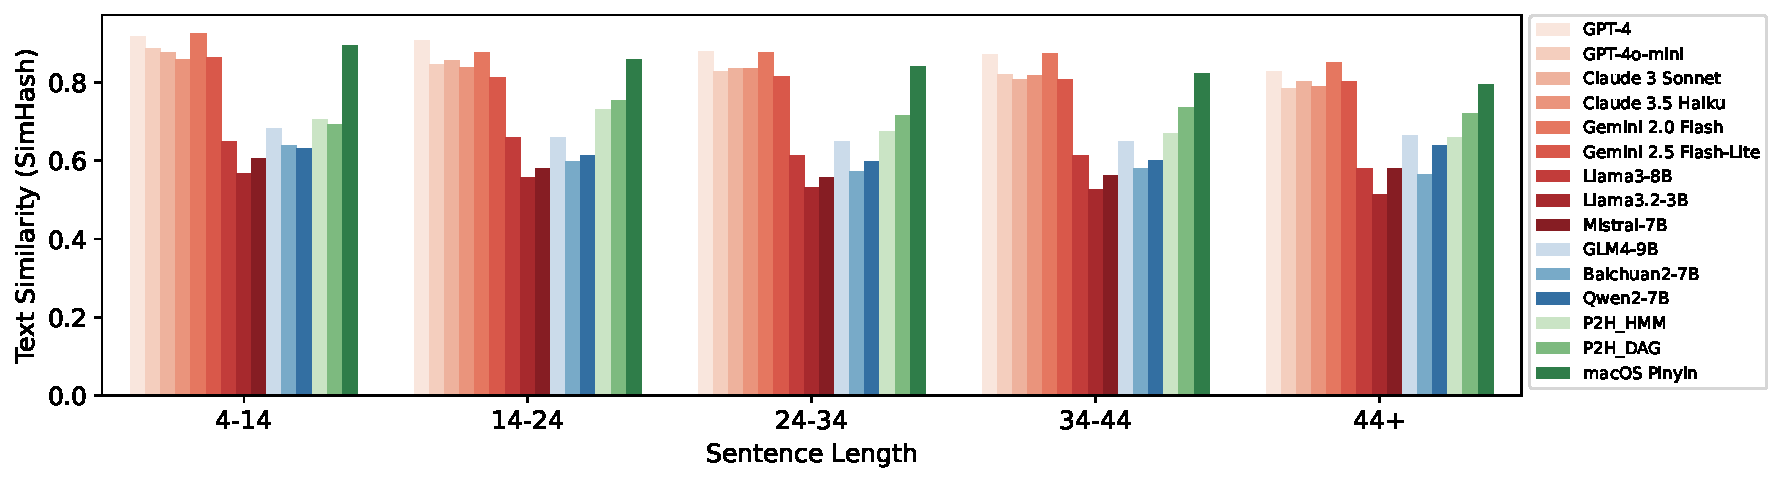
\includegraphics[width=\textwidth]{../figures/csg_textsim_wl.pdf}\\
    \vspace{2mm}
    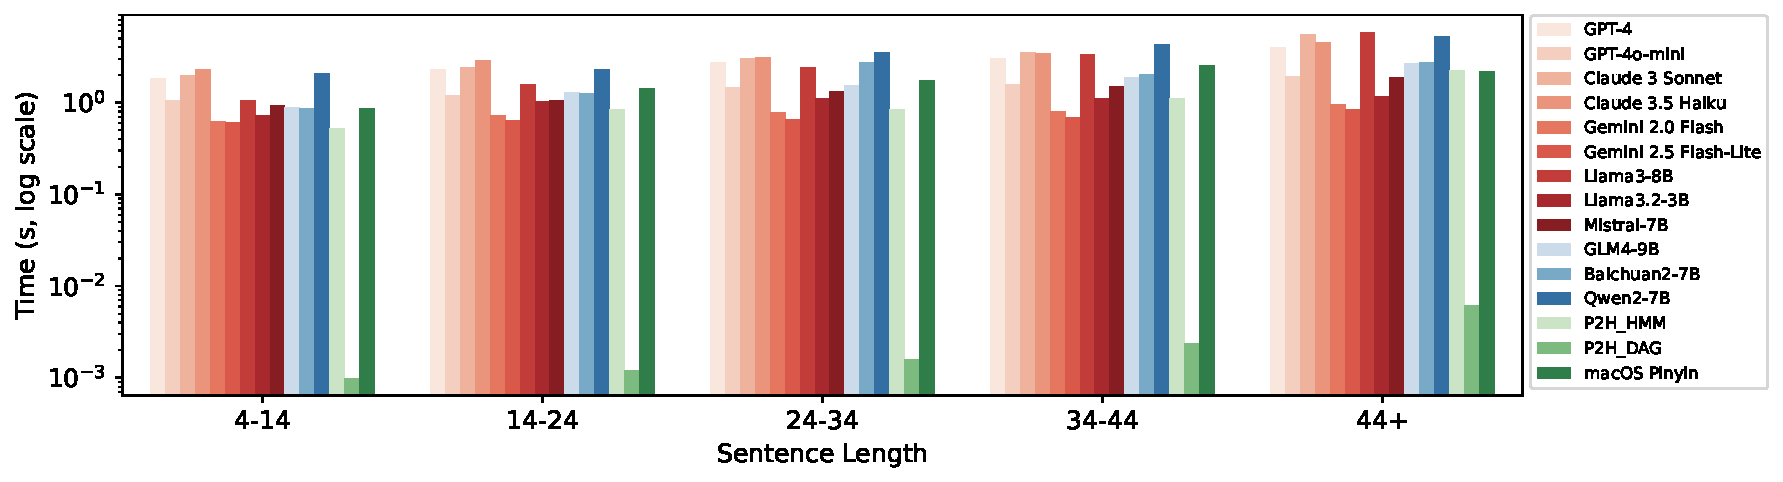
\includegraphics[width=\textwidth]{../figures/csg_time_wl.pdf}
    \caption{Average text similarity (SimHash) and completion time vs. sentence length for Chinese Sentence Generation.}
    \label{fig:csg_wl}
\end{figure*}

\begin{figure*}[h!]
    \centering
    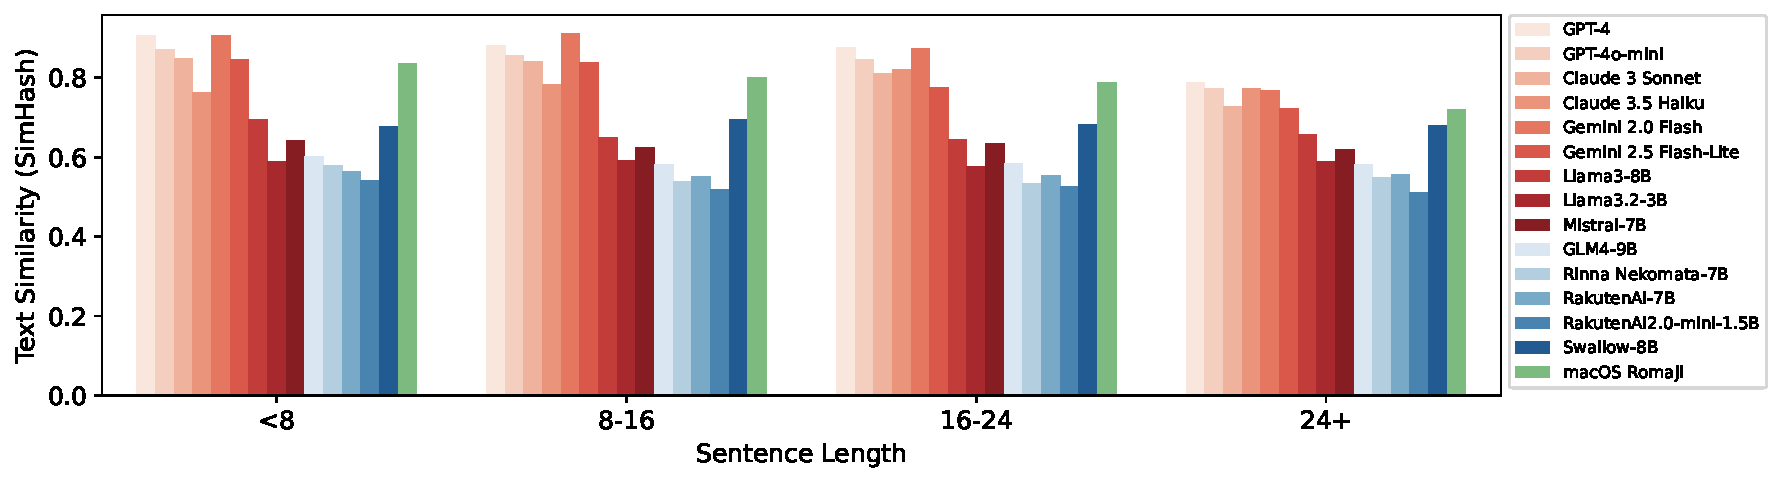
\includegraphics[width=\textwidth]{../figures/jsg_textsim_wl.pdf}\\
    \vspace{2mm}
    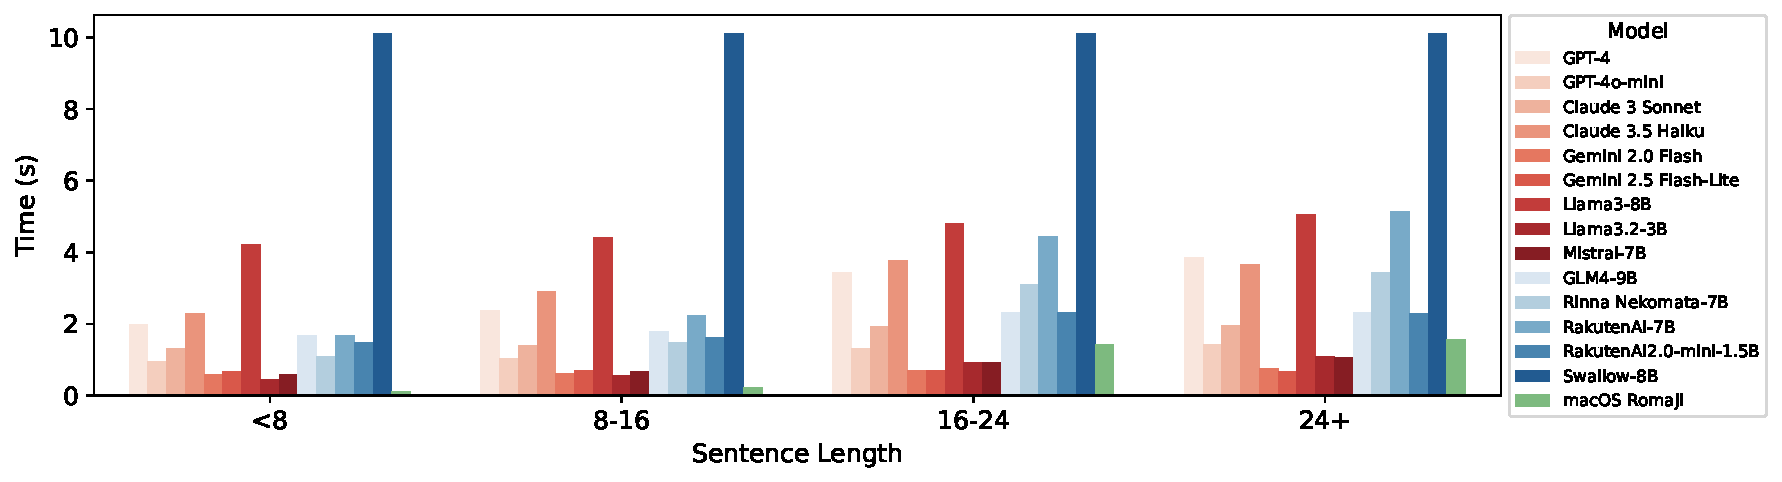
\includegraphics[width=\textwidth]{../figures/jsg_time_wl.pdf}
    \caption{Average text similarity (SimHash) and completion time vs. sentence length for Japanese Sentence Generation.}
    \label{fig:jsg_wl}
\end{figure*}

\subsection{Performance vs. Noise Level in Error Correction}

Figures~\ref{fig:cec_pinyin_noise} and \ref{fig:jec_char_noise} are crucial for assessing model robustness, showing how performance degrades as the number of errors in the source text increases.

For Chinese pinyin error correction (Figure~\ref{fig:cec_pinyin_noise}), the accuracy plot demonstrates the remarkable resilience of top-tier LLMs. Models like GPT-4o and Gemini 2.0 Flash maintain a very high SimHash score even when faced with 4 or 5 errors, with only a marginal drop in performance. This indicates a strong ability to infer user intent from heavily corrupted phonetic input. In contrast, the performance of smaller offline models like Llama3-8B and Mistral-7B starts lower and degrades more quickly, suggesting they are more easily thrown off by multiple errors. The completion time plot shows that for most models, the time taken does not significantly increase with the number of errors, suggesting that the core computational cost is tied to processing the sentence length, not the difficulty of the correction.

For Japanese character error correction (Figure~\ref{fig:jec_char_noise}), the trends are similar. The elite performance of GPT-4o is visually striking, with its accuracy remaining almost flat and near-perfect regardless of the number of errors. The {OpenNMT} baseline, while strong with 1-2 errors, shows a more noticeable decline in performance as the noise level increases, highlighting the superior robustness of the top LLM's contextual reasoning. This visual evidence strongly supports the conclusion that large-scale LLMs are not just more accurate at error correction, but also more reliable under challenging conditions.

\begin{figure*}[h!]
    \centering
    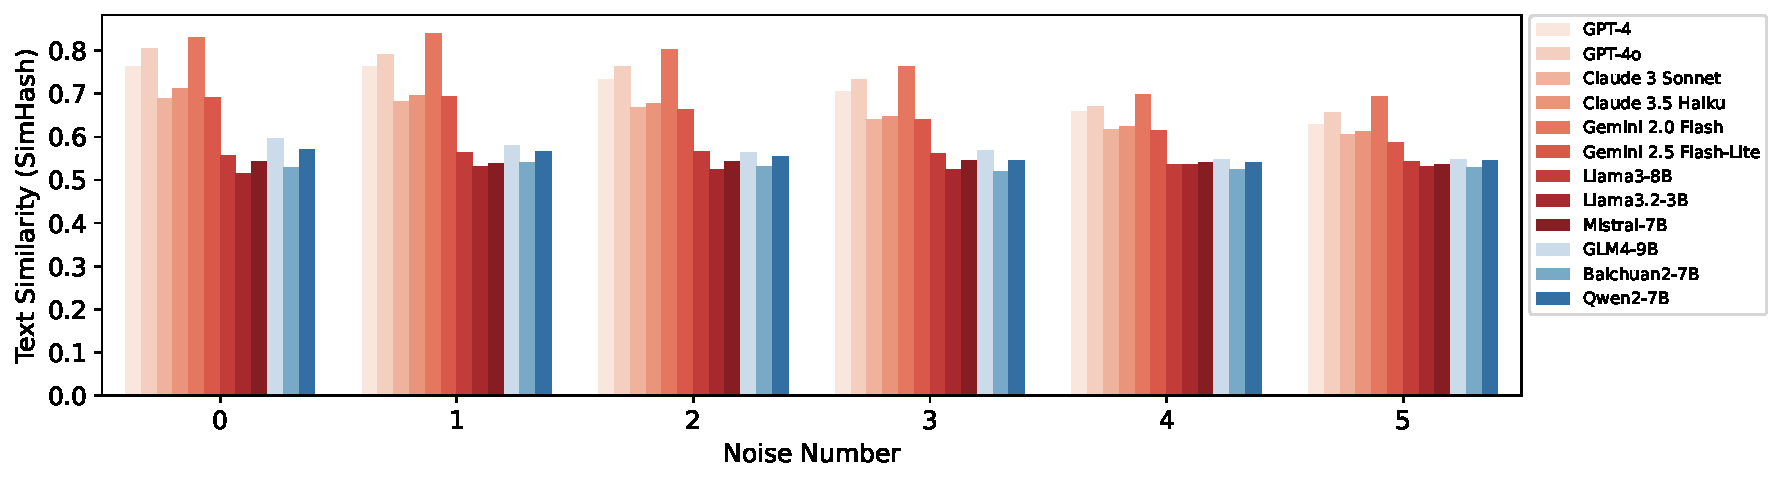
\includegraphics[width=\textwidth]{../figures/cec_pinyin_textsim_noise.pdf}\\
    \vspace{2mm}
    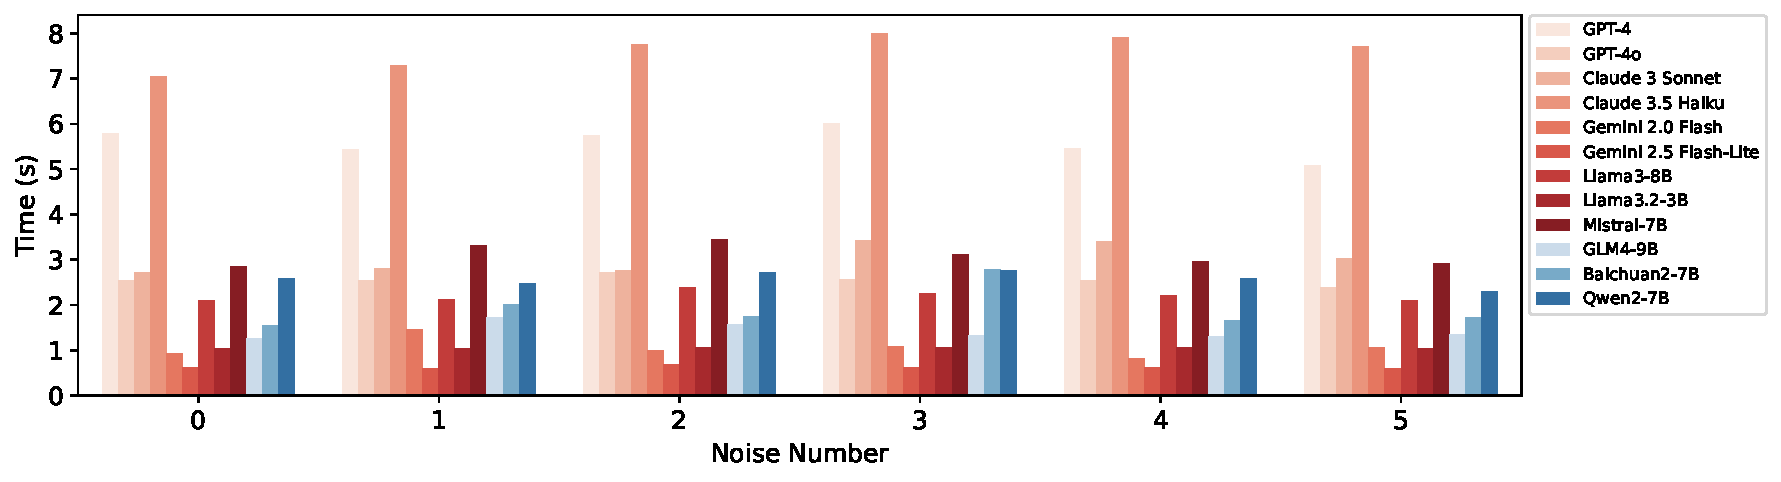
\includegraphics[width=\textwidth]{../figures/cec_pinyin_time_noise.pdf}
    \caption{Average text similarity (SimHash) and completion time vs. number of errors for Chinese Pinyin Error Correction.}
    \label{fig:cec_pinyin_noise}
\end{figure*}

\begin{figure*}[h!]
    \centering
    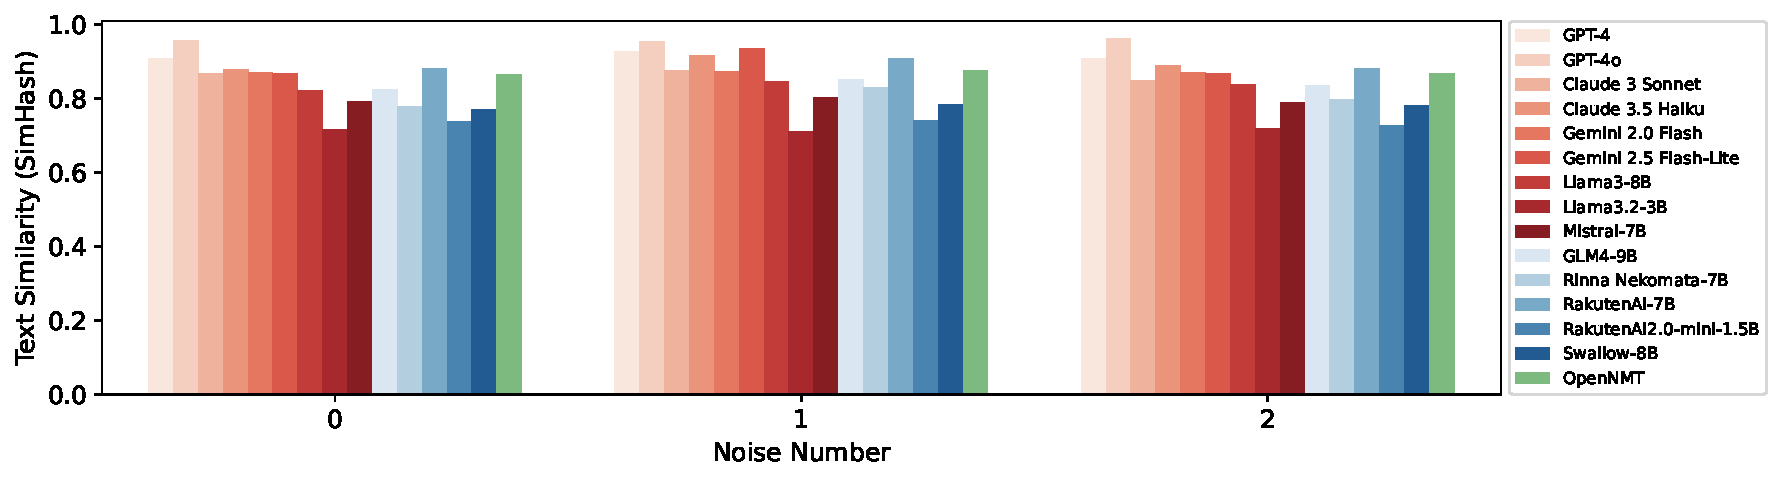
\includegraphics[width=\textwidth]{../figures/jec_char_textsim_noise.pdf}\\
    \vspace{2mm}
    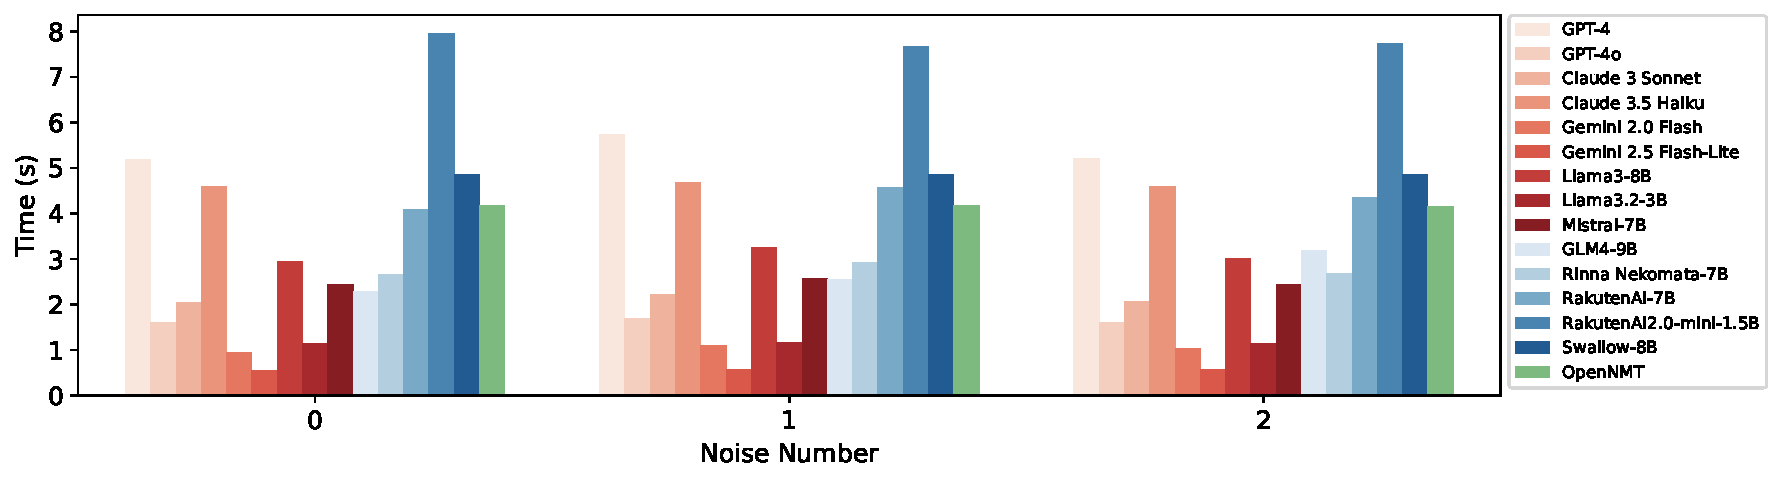
\includegraphics[width=\textwidth]{../figures/jec_char_time_noise.pdf}
    \caption{Average text similarity (SimHash) and completion time vs. number of errors for Japanese Character Error Correction.}
    \label{fig:jec_char_noise}
\end{figure*}

\begin{figure*}[h!]
    \centering
    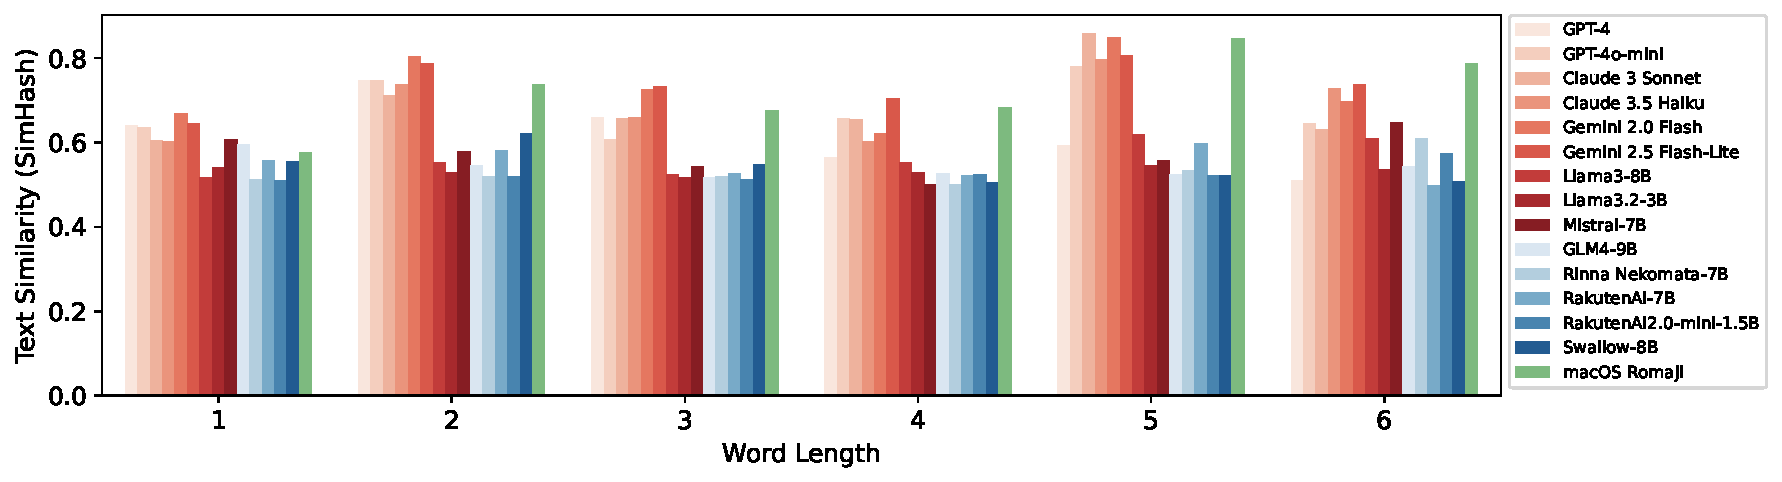
\includegraphics[width=\textwidth]{../figures/jwg_kanji_textsim_wl.pdf} \\
    \vspace{2mm}
    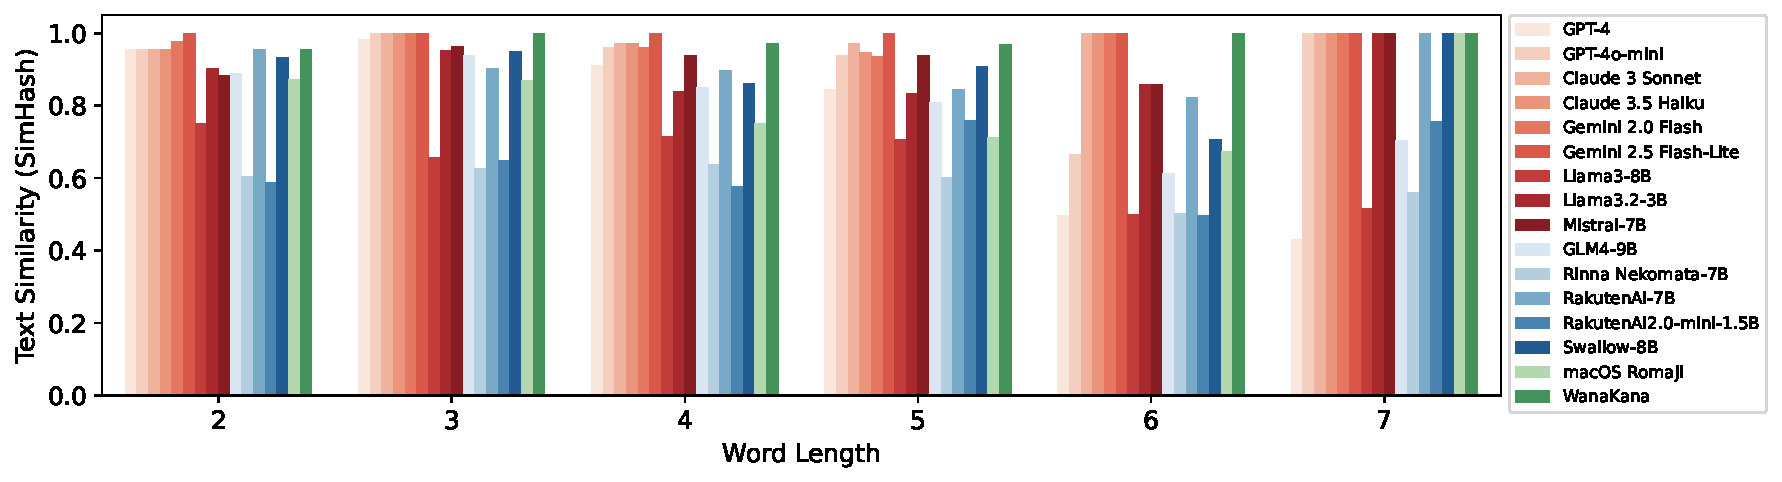
\includegraphics[width=\textwidth]{../figures/jwg_hira_textsim_wl.pdf} \\
    \vspace{2mm}
    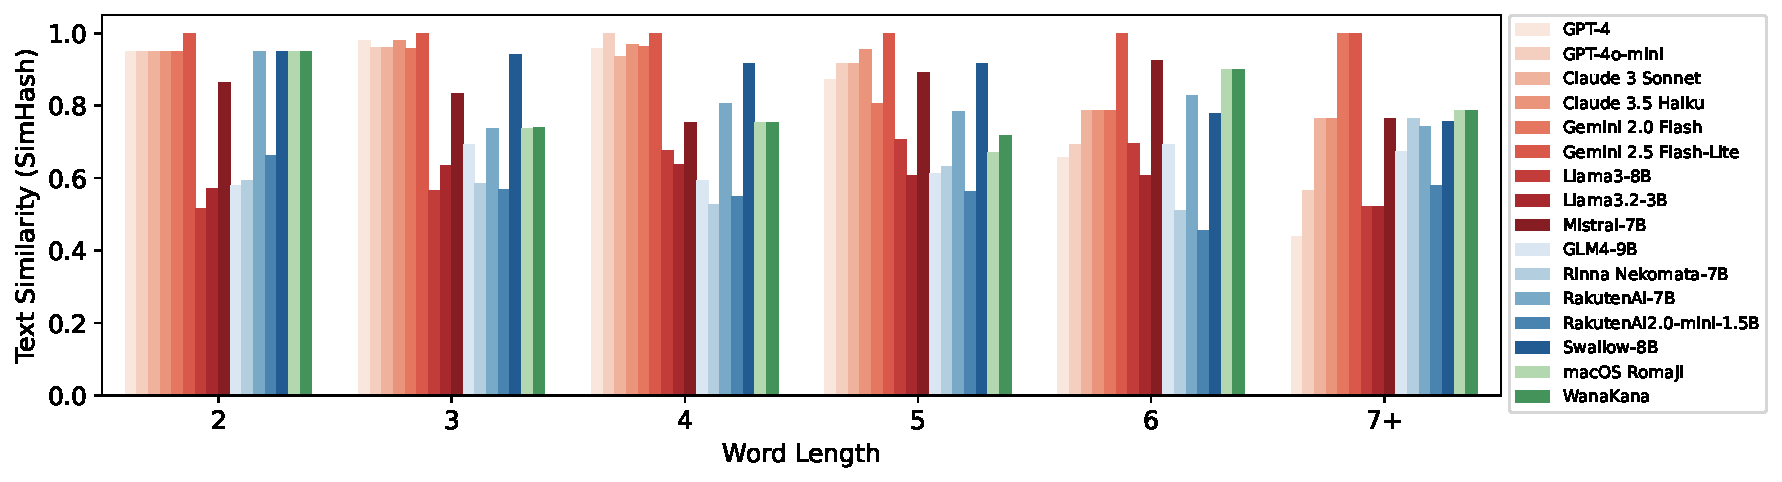
\includegraphics[width=\textwidth]{../figures/jwg_kata_textsim_wl.pdf}
    \caption{Average text similarity (SimHash) vs. word length for Japanese Word Generation, broken down by primary script type: Kanji (top), Hiragana (middle), and Katakana (bottom).}
    \label{fig:jwg_script}
\end{figure*}
\subsection{Japanese Word Generation by Script Type}

Figure~\ref{fig:jwg_script} provides a unique and insightful breakdown of model performance on Japanese word generation based on the primary script of the target word: Kanji, Hiragana, or Katakana. This analysis isolates the specific challenges within Japanese text input.

The plots clearly show that Kanji generation is the most difficult task for all models. The overall SimHash scores are lowest for Kanji, and the performance gap between the top models (like Gemini 2.0 Flash) and weaker models is at its widest. This visually confirms that Kanji disambiguation, which requires deep semantic understanding to differentiate between homophones, is the primary hurdle in Japanese IMEs.

In stark contrast, performance on Hiragana and Katakana is much higher and more uniform across most models. For these purely phonetic scripts, the task is closer to a simple transliteration, and even smaller models perform well. The macOS Romaji baseline, in particular, excels at these tasks, which explains its strong overall baseline scores in the main tables. This visual breakdown is critical: it demonstrates that simply averaging performance on ``Japanese'' can be misleading. The true test of an advanced Japanese IME lies in its ability to correctly generate Kanji, and it is on this specific sub-task that the leading LLMs demonstrate their most significant advantage over traditional methods.


\end{document}

%%% Local Variables:
%%% mode: latex
%%% TeX-master: t
%%% End:
